\documentclass[draft]{agujournal2019}

\newcommand{\todo}[1]{\textcolor{red}{\textbf{(#1)}}}

\usepackage{amsmath}

\linenumbers
\journalname{Journal of Advances in Modeling Earth Systems (JAMES)}

\begin{document}

\title{Responses to Humidity and Temperature Perturbations in High-Resolution Simulations of Convection}

\authors{Timothy H. Raupach\affil{1,2}, Chimene L. Daleu\affil{3}, Robert S.
Plant\affil{3}, Steven S.Sherwood\affil{1,2}, and Yi-Ling Hwong\affil{4}}

\affiliation{1}{Climate Change Research Centre, University of New South Wales, Sydney, Australia}
\affiliation{2}{ARC Centre of Excellence for Climate Extremes}
\affiliation{3}{Department of Meteorology, University of Reading, Reading, United Kingdom}
\affiliation{4}{Institute of Science and Technology Austria, Vienna, Austria}

\correspondingauthor{Timothy H. Raupach}{timothy.h.raupach@gmail.com}

\begin{keypoints}
\item \todo{1-3 key points, $\leq$ 140 characters each}
\end{keypoints}

\justifying
\begin{abstract}
\todo{Abstract\ldots}
\end{abstract}

\section*{Plain Language Summary}
\todo{Plain language summary\ldots}

\section{Introduction}

In the atmosphere, deep convection refers to overturning circulations, formed by
bouyant air, that reach the tropopause \cite{Wallace_2006}. Deep convection is
associated with the formation of severe thunderstorms \cite{Doswell_2001}. While
deep convection covers only a small proportion of the Earth's surface at any one
time, its resulting storms produce a large proportion of the Earth's rainfall
\cite{Wallace_2006}. Deep convection also warms the atmosphere and balances
radiative cooling, such that on average the tropics remain in
radiative-convective equilibrium (RCE) \cite{Manabe_JAS_1964}. These important
effects mean that models such as global and regional climate models
(respectively GCMs and RCMs) need to take deep convection into account. However,
models often use horizontal grid spacings that are much larger than the
horizontal scale of convection, meaning that they are unable to resolve
individual convective cells. In this case, the model must account for the
effects of convection -- such as its heating effect or rain it may produce -- by
parameterising the sub-grid convection that it can not explicitly resolve. Such
parameterisations are called convection schemes. 

Many different convection schemes have been produced, each with different
strengths, weaknesses, and assumptions \cite<e.g.>{Kain_JAS_1990,
Arakawa_JC_2004, Rio_CCCR_2019, Lin_AO_2022}. Such are the differences between
these schemes, and so high is the sensitivity of models to convective cloud
physics \cite<e.g.>{Emanuel_JAS_1999}, that convection parameterisation is a
leading source of uncertainty in model outputs \cite<e.g.>{Hwong_JAMES_2021}. It
is difficult to compare convection schemes, since traditional methods in which
simulated outputs are compared with observations \cite<e.g.>{Grell_ACP_2014,
Kwon_MWR_2017, Zhang_JC_2017, Zhang_MWR_2011} rely on observation selection and
accuracy \cite{Hwong_JAMES_2021}.

The mathematical framework proposed by \citeA{Kuang_JAS_2010} uses linear
response functions to compare model behaviour via assessment of the models'
responses to small perturbations in the larger-scale atmospheric properties. In
this method, the responses of the model (and thus the convection scheme) are
examined in idealised simulations under different small perturbations to the
humidity and temperature tendencies. The idea is that although there are many
non-linear processes in convection, the statistics of the cumulus ensemble as a
whole can be well-described by smooth linear functions that describe how the
ensemble reacts to small changes in its large-scale environment
\cite{Kuang_JAS_2010}. An advantage of this approach is that the responses of
the model to perturbations can be distilled by the linear response functions,
which describe the model behaviour well enough to, for example, describe the
dynamics of convectively coupled waves \cite{Kuang_JAS_2010}. Even if a linear
approximation is inadequate for fully describing convection, it can be a useful
first-order characterization.

The linear response framework was applied to single column models (SCMs) by
\citeA{Herman_JAMES_2013} specifically for the purpose of testing two convection
schemes. \citeA{Hwong_JAMES_2021} used the framework to evaluate convection,
planetary boundary, and microphysics schemes' responses to perturbations in
SCMs. They showed that the results isolate the convection scheme in at least the
tested SCMs, and examined a large number of schemes in actual use
\cite{Hwong_JAMES_2021}. The technique allows for efficient comparison of
different model setups, but does not answer the question of which setup is most
accurate. To answer this question, study of the linear responses of a model that
uses the fewest possible parameterisations is required. \citeA{Kuang_JAS_2010}
performed a large ensemble of large eddy simulation (LES) runs, but used a
rather coarse resolution of 4 km and only a single LES model, the System for Atmospheric Modelling \cite<SAM, e.g.>{Khairoutdinov_JAS_2003}.

In this study, we ran perturbation experiments on models at high resolution and
compared the results to perturbations run at lower resolution, to attempt to
produce benchmark results and determine the effect of the planetary boundary
layer (PBL) scheme when convection is resolved explicitly. The key question is
whether the response of a cloud-resolving model (CRM) or large eddy simulation
(LES) to a forcing perturbation is robust, or whether it is sensitive to
modelling decisions that one might make in high-resolution modelling, such as
the grid length, model dynamics, or the microphysics used. A related question is
whether the response is dominated by the modelled convection itself, or whether
it might be sensitive to the specification of surface properties in an idealized
modelling setting. All this is important in being able to judge differences
between models in \citeA{Hwong_JAMES_2021}. Here we aim to answer whether
differences seen between models point to errors in one or more convection
parameterizations, or are within the uncertainties found in different credible
LES simulations. 

The rest of this manuscript is organised as follows. In Section
\ref{sec:methods} we introduce the methods we used including modelling setups.
Results are shown in Section \ref{sec:results} and conclusions are drawn in
Section \ref{sec:conclusions}.

\section{Methods}
\label{sec:methods}

We used two models in this work: the Advanced Research (AR) version of the
Weather Research and Forecasting (WRF) model, version 4.1.4
\cite{Skamarock_2019}, and the Met Office/NERC Cloud Model
\cite<MONC,>{Brown_2020} as used in \citeA{Daleu_QJRMS_2023}.

\subsection{Common Model Settings}

Both models were used to simulate convection at high resolution over a water
surface with periodic boundary conditions. The models used a constant sea
surface temperature (SST) of 301.15 K. This value is a little different from
that used in \citeA{Kuang_JAS_2010} but matches \citeA{Hwong_JAMES_2021}. We
used idealised radiation as in \citeA{Herman_JAMES_2013} and
\citeA{Hwong_JAMES_2021}, but unlike \citeA{Kuang_JAS_2010} who used interactive
radiation. Following \citeA{Herman_JAMES_2013}, the radiative cooling tendency
was $\theta_{tend,rad} = \theta_t/\Pi$ K day$^{-1}$, where $\Pi$ is the Exner
function that converts temperature to potential temperature, and $\theta_t$ is a
temperature tendency set as \todo{double check in code for WRF}

\begin{align}
 \theta_t = \begin{cases}
    -1.5\; \textrm{K day}^{-1} & \textrm{if}\, p \geq 200\; \textrm{hPa}, \\
    0\; \textrm{K day}^{-1} & \textrm{if}\, p \leq 100\; \textrm{hPa}, \\
    -1.5 + \frac{1.5 (p-100)}{100}\; \textrm{K day}^{-1} & \textrm{if}\, 100 < p < 200\; \textrm{hPa}. \\
 %* $t$'s value varies linearly between -1.5 and 0 K day$^{-1}$ from 100 to 200 hPa.
 \end{cases}
\end{align}

We used idealised evaporation as in \citeA{Chua_GRL_2019}, with minor
differences. We used a constant surface wind speed of $W_s = 4.8$ m s$^{-1}$,
following \citeA{Hwong_JAMES_2021} who used the same approach with a fixed value
of 0.001 for the surface exchange coefficient. While the wind speed here and in
\citeA{Hwong_JAMES_2021} was slightly different from that of
\citeA{Kuang_JAS_2010}, the important quantity is the product of the wind with
the surface exchange coefficient, and the exchange coefficient value in
\citeA{Kuang_JAS_2010} was not stated. Here we used a fixed value of 0.005 for
this quantity \todo{double check for WRF and MONC}. Level-mean horizontal winds
were relaxed to $u = 0$ m s$^{-1}$ and $v = 5$ m s$^{-1}$, where $u$ is the
zonal and $v$ is the meridional wind component, respectively, with a three-hour
relation time.

For each resolution, the models were run until they reached radiative convective
equilibrium (RCE) at time $t_1$. After RCE was reached, small perturbations in
the imposed temperature or moisture forcings were introduced, while a control
was run with no perturbations, and the models were allowed to again reach RCE at
time $t_2$. For a time block after $t_2$, domain-mean atmospheric profiles for
the perturbed runs were subtracted from the domain mean profiles in the control
runs to examine the differences made by the perturbations. In the following two
sections we examine the model-specific setups for WRF and MONC, respectively.

\subsection{WRF}

WRF was run on a 20 $\times$ 20 km$^2$ domain for horizontal grid spacings of 4
km, 1 km and 100 m. The runs at 4 km and 1 km grid resolution used 74 grid
points in the vertical while the run at 100 m grid spacing used 370 vertical
grid points. The parameterisations used are summarised in Table
\ref{tab:WRF_schemes}. The model timestep was set to 6 s for 4 km and 1 km grid
spacing and 1 s for 100 m grid spacing, and outputs were recorded hourly for the
1 km and 4 km cases, and at 2 hour resolution for the 100 m cases. For the runs
with 1 km and 4 km grid spacing, the models were initialised using a
Radiative-Convective Equilibrium Model Intercomparison Project (RCEMIP) profile
\cite{Wing_GMD_2018}. For the runs at 100 m grid spacing, the model was
initialised using the mean RCE model state from the 1 km control run, so that
the LES runs started near RCE to reduce computation time. Temperature and water
vapour mixing ratio in the stratosphere were relaxed to the initial profile
values to avoid model drift, as suggested by \citeA{Herman_JAMES_2013}.
Relaxation was applied above 160 hPa with the inverse relaxation constant
increasing linearly from $1/\tau = 0$ day$^{-1}$ at 160 hPa to $1/\tau = 0.5$
day$^{-1}$ at and above 100 hPa \cite{Herman_JAMES_2013}. Full diffusion
(\texttt{diff\_opt = 2}) was used at all resolutions; at 4 km and 1 km
resolutions, horizontal diffusion was diagnosed from deformation and vertical
diffusion was assumed done by the planetary boundary layer scheme
(\texttt{km\_opt = 4}) while the simulations at 100 m used a prognostic equation
(\texttt{km\_opt = 2}) for turbulent kinetic energy \cite{Skamarock_2019}. Per
resolution, restarts were synchronised between perturbation and control runs to
ensure consistency.

\begin{table}[t]
    \caption{Parameterisations used in the WRF simulations. These schemes were
     used for all resolutions, with the exception of the boundary layer scheme
     which was enabled only for the 4 km and 1 km simulations. No convection
     parameterisation was used.}
    \label{tab:WRF_schemes}
    \centering
    \begin{tabular}{lll}
    \hline
    \textbf{Parameterisation} & \textbf{Scheme} & \textbf{Reference} \\
    \hline
    Microphysics & Thompson & \citeA{Thompson_MWR_2008} \\
    Boundary layer & YSU & \citeA{Hong_MWR_2006} \\
    Surface layer & Revised MM5 & \citeA{Jimenez_MWR_2012} \\
    Land surface & Thermal diffusion & \citeA{Dudhia_1996} \\
    \hline
    % \multicolumn{2}{l}{$^{a}$Footnote text here.}
    \end{tabular}
\end{table}

We used idealised evaporation as in \citeA{Chua_GRL_2019} and
\citeA{Hwong_JAMES_2021}, with a fixed surface wind speed and the drag
coefficient assumed to be 0.001. Then surface heat flux (SH) was calculated
using modified Eq. 1 from \citeA{Chua_GRL_2019}, such that

$$
\textrm{SH} = 0.001 \rho_a W c_p (T_s - T_a),
$$

\noindent where $\rho_a$ (kg m$^{-3}$) is the near surface air density, $T_s$
(K) is surface temperature (we use SST), and $T_a$ (K) is the near-surface air
temperature. We used 

$$
T_a = T_l \left(\frac{p_s}{p_l}\right)^{\frac{R_d}{c_p}},
$$

\noindent where $T_l$ (K) is the temperature at the first model level above the
surface, $p_s$ (hPa) is surface pressure, $p_l$ (hPa) is pressure at the first
model level, $c_p$ (J kg$^{-1}$ K$^{-1}$) is the specific heat capacity of dry
air at constant pressure, and $R_d$ (J kg$^{-1}$ K$^{-1}$) is the gas constant
for dry air. Latent heat flux (LH) was calculated using modified Eq. 2 from
\citeA{Chua_GRL_2019}, such that

$$
\textrm{LH} = 0.001 \rho_a W L (q_{sat} - q_a),
$$

\noindent where $L$ is the typical latent heat of vaporization of water,
$q_{sat}$ is the saturated water vapour mixing ratio at $T_s$ (we use WRF's
``ground saturated mixing ratio'') and $q_a$ is the water vapour mixing ratio at
the lowest model level. Note that while \citeA{Chua_GRL_2019} assumed that air
density near the surface is 1 kg m$^{-3}$, we used the near-surface density
value produced by WRF (around 1.16 kg m$^{-3}$).

Because the pressure levels in the WRF model were not exactly at the points
around which we want to perturb, we adapted the form of perturbations used by
\citeA{Herman_JAMES_2013} so that only the Gaussian portion of the perturbation
function is used, and instead of selecting a level $k$ a pressure $p_p$ (hPa)
around which to perturb is selected. The perturbation function used in the WRF
simulations for the $i$th model level was

$$
f_i = \exp\left[ - \left( \frac{p_p - p_i}{75 \textrm{hPa}}\right)^2 \right],
$$

\noindent where $p_p$ (hPa) is the chosen perturbation pressure and $p_i$ is the
pressure at level $i$. We calculated the spatial means per interpolated model
pressure level, per time step. The temporal average of these mean profiles over
the RCE period was calculated for each run for comparison.

\subsection{MONC}

MONC was run on a 64 $\times$ 64$^2$ domain for grid spacings of 1 km, 500 m,
and 250 m. The MONC setup was similar to that used in \citeA{Daleu_QJRMS_2023}:
the domain height was 20 km with a Newtonian damping layer above 16 km; we used
bi-periodic lateral boundary conditions; the 3D Smagorinsky scheme was used to
calculate subgrid turbulent eddy fluxes; and the Cloud AeroSol Interactive
Microphysics \cite<CASIM, see>[and references therein for previous
uses]{Daleu_QJRMS_2023} scheme represented cloud processes. The model time step
varied between 1 and 2 seconds. Perturbations were made using a combinations of
the delta and Gaussian functions, as in Equation 4 of \citeA{Herman_JAMES_2013}.
We used an idealized treatment of evaporation in the sense that a constant
near-surface wind speed of 5 m s$^{-1}$ was imposed \todo{confirm if 5 or 4.8
for WRF}. For pressure levels less than 160 hPa, temperature and moisture fields
were relaxed to the values of a previous RCE run, following
\cite{Herman_JAMES_2013} \todo{check if same for WRF and if so move to common
settings}.

\subsection{Perturbations to Temperature and Humidity}

Constant perturbations were applied to potential temperature or water vapour
tendencies at given model levels. Given computational constrains, not all
perturbations were applied in all runs.  Table \ref{tab:pert_runs} shows which
perturbations were applied to which model runs. For the WRF runs, we used the
results of \cite{Hwong_JAMES_2021} \todo{YLH please check this is the right
reference} to find two levels on which perturbations provided the most
information about perturbations across other levels (not shown here). The two
``most representative'' levels were a low (850 hPa) and a high (412 hPa)
perturbation level, which we use here in the high-resolution WRF runs. Other
levels on which perturbations were applied were 415 hPa (MONC only), 500 hPa,
600 hPa, and 730 hPa. For simplicity of comparison, in the following we refer to
the MONC results for a perturbation at 415 hPa as results for a perturbation at
412 hPa.

{
\begin{table}
    \centering
    \caption{Perturbations appled by variable, model, and grid spacing. Here,
    412 hPa refers to 412 hPa in the WRF runs but 415 hPa in the MONC runs. A
    $\bullet{}$ symbol indicates the given model was run with the given
    resolution and perturbation. $T$ is \todo{potential} temperature in K and
    $q$ is water vapour mixing ratio in kg kg$^{-1}$.}
    \label{tab:pert_runs}
    \renewcommand{\arraystretch}{0.6}
    \begin{tabular}{lllccccc}
        \multicolumn{3}{r}{\textbf{Model}} & \multicolumn{2}{c}{\textbf{WRF}} & \multicolumn{3}{c}{\textbf{MONC}} \\
        \multicolumn{3}{r}{\textbf{Grid spacing}} & 4 and 1 km & 100 m & 1 km & 500 m & 250 m \\
        
        \textbf{Variable} & \textbf{Perturbation} & \textbf{Level} & & & & & \\
        \hline
        % T +
        T & $+0.5$ K & 412 hPa & $\bullet{}$ & $\bullet{}$ & $\bullet{}$ &  & $\bullet{}$ \\
        & & 500 hPa & $\bullet{}$ & & $\bullet{}$ & $\bullet{}$ & $\bullet{}$ \\
        & & 600 hPa & $\bullet{}$ & & $\bullet{}$ &  & $\bullet{}$ \\
        & & 730 hPa & $\bullet{}$ & & $\bullet{}$ &  & $\bullet{}$ \\
        & & 850 hPa & $\bullet{}$ & $\bullet{}$ & $\bullet{}$ & $\bullet{}$ & $\bullet{}$ \\
        % T -
        & $-0.5$ K & 412 hPa & $\bullet{}$ & $\bullet{}$ & $\bullet{}$ &  & $\bullet{}$ \\
        & & 500 hPa & $\bullet{}$ & & $\bullet{}$ &  & $\bullet{}$\\
        & & 600 hPa & $\bullet{}$ & & $\bullet{}$ &  & $\bullet{}$ \\
        & & 730 hPa & $\bullet{}$ & & $\bullet{}$ &  & $\bullet{}$ \\
        & & 850 hPa & $\bullet{}$ & $\bullet{}$ & $\bullet{}$ &  & $\bullet{}$ \\
        \hline
        % q +
        q & $+0.0002$ kg kg$^{-1}$ & 412 hPa & $\bullet{}$ & $\bullet{}$ & $\bullet{}$ &  &  \\
        & & 500 hPa & $\bullet{}$ & & $\bullet{}$ & $\bullet{}$ & $\bullet{}$ \\
        & & 600 hPa & $\bullet{}$ & & $\bullet{}$ &  &  \\
        & & 730 hPa & $\bullet{}$ & & $\bullet{}$ &  &  \\
        & & 850 hPa & $\bullet{}$ & $\bullet{}$ & $\bullet{}$ & $\bullet{}$ & $\bullet{}$ \\
        % q -
        & $-0.0002$ kg kg$^{-1}$ & 412 hPa & $\bullet{}$ & $\bullet{}$ & $\bullet{}$ &  &  \\
        & & 500 hPa & $\bullet{}$ & & $\bullet{}$ &  &  \\
        & & 600 hPa & $\bullet{}$ & & $\bullet{}$ &  &  \\
        & & 730 hPa & $\bullet{}$ & & $\bullet{}$ &  &  \\
        & & 850 hPa & $\bullet{}$ & $\bullet{}$ & $\bullet{}$ &  &  \\
        \hline
    \end{tabular}
\end{table}
}

\section{Results}
\label{sec:results}

\subsection{Radiative-Convective Equilibrium Mean State}

We used plots of spatially-averaged precipitable water by time to determine when
the models had reached RCE. Figure \ref{fig:rce_pw} shows precipitable water by
time for the WRF runs and columnar water vapour by time for the MONC runs. For
the WRF runs, at 4 km grid spacing the RCE state had a precipitable water (PW)
of $\sim$40 mm, which rose to $\sim$44 mm at 1 km grid spacing and $\sim$42 mm
at 100 m grid spacing. For the MONC runs, \todo{\ldots}.

\begin{figure}[pth]
    \noindent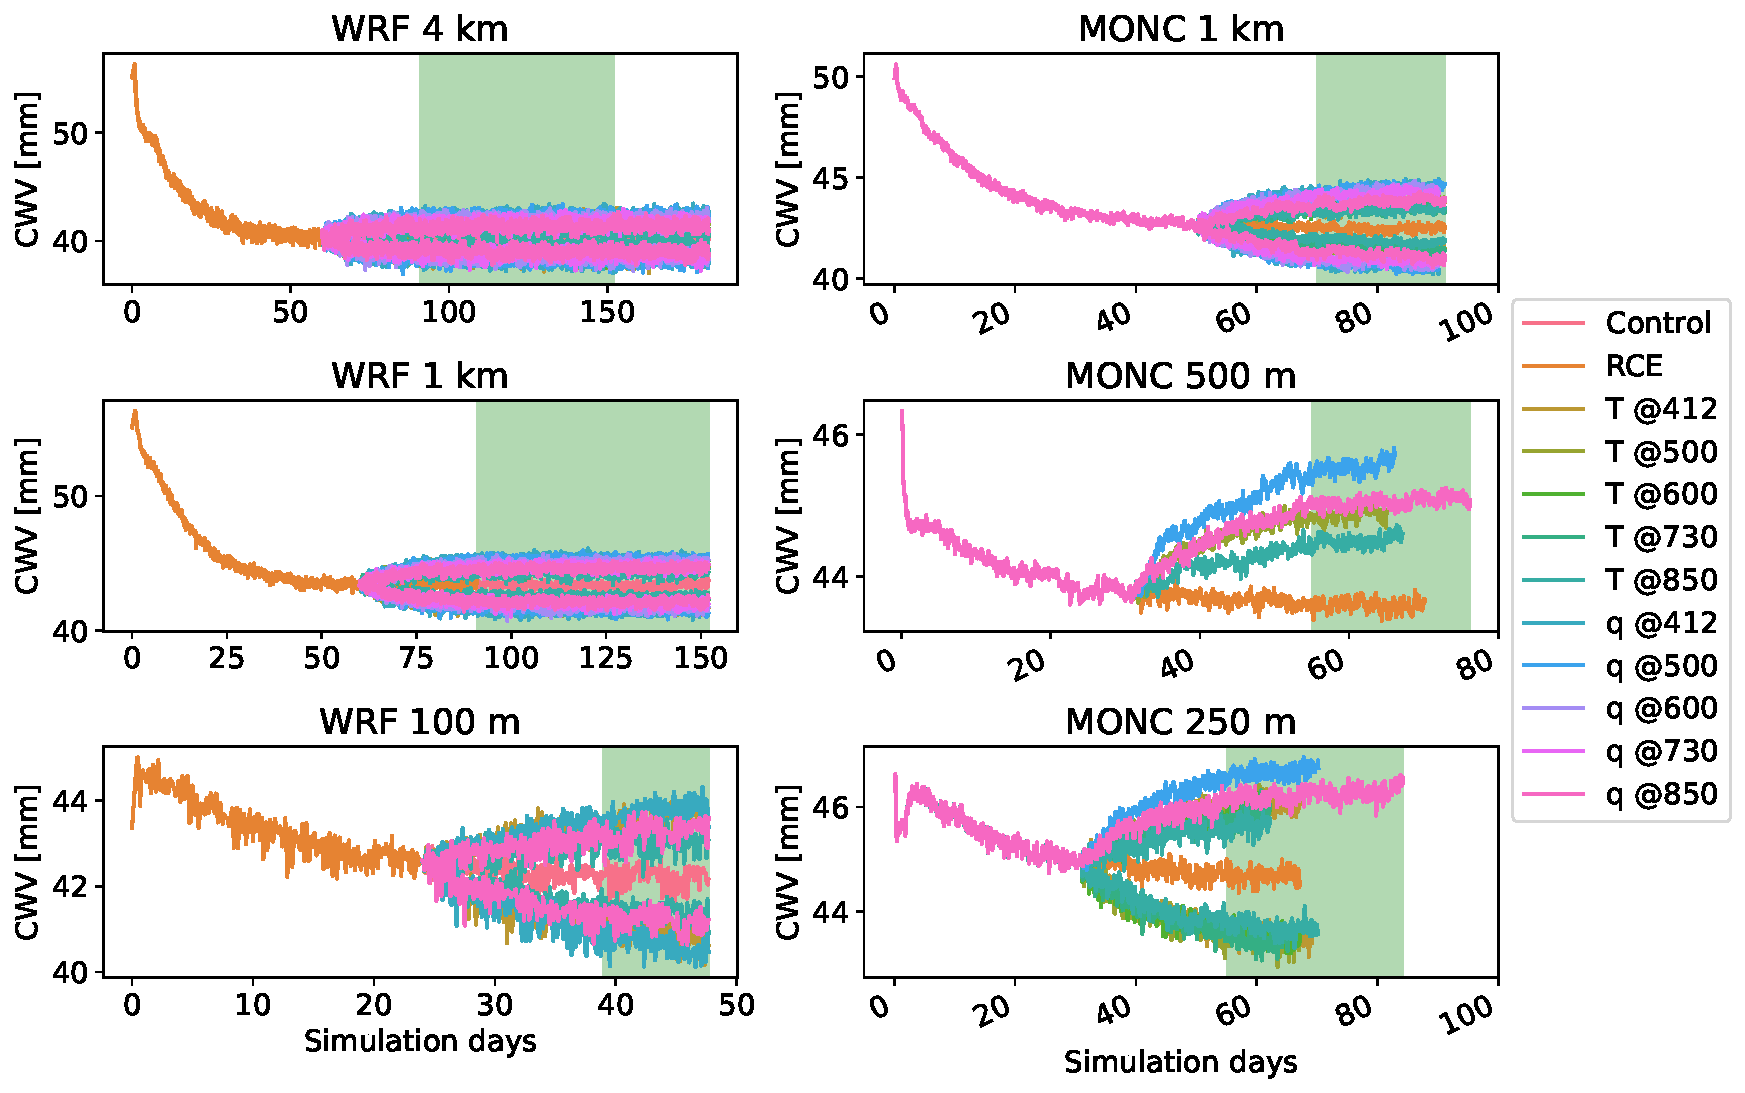
\includegraphics[width=\textwidth]{figures/runs_timeseries.pdf}
    \caption{Timeseries of water content in WRF and MONC. For WRF, the plots
    show timeseries of the spatial mean precipitable water by grid spacing. For
    MONC, the plots show timeseries of spatial mean column water vapour by grid
    spacing. RCE runs were computed until precipitable water content/columnar
    water content stabilised and the model was at RCE. At this point the
    perturbations were introduced and the model was run until all perturbed runs
    were also at RCE. The parts of the time axes highlighted in green show the
    ``RCE region'' over which mean profiles were calculated for comparison. For
    the MONC runs, the highlighted region shows the maximum range of RCE
    regions, since RCE regions were defined as the last 20 days in each
    simulation for 1 km runs and the last 10 days in each simulation for the 500
    m and 250 m runs. Note that to reduce the number of colours required,
    positive and negative perturbations per variable and perturbation pressure
    use the same colour.}
    \label{fig:rce_pw}
\end{figure}

Mean profiles from the control run in RCE are shown in Figure
\ref{fig:rce_profiles}. The mean states are similar across the two models,
especially within the context of larger inter-model comparisons of RCE states
\todo{cite examples}. To some extent the similarities may be due to the
idealised treatment of radiation and evaporation used here. Moisture content
generally increases with increasing resolution, although the changes are modest
at 1 km and higher-resolution grid spacing. MONC is marginally more moist than
WRF. The additional moisture at finer resolutions appears in the lower part of
the free troposphere above about 900 hPa, which we hypothesise is the result of
some transport from shallow convection. Mean wind profiles for the 100 m run,
which had increased vertical resolution than, and was temporally shorter than
the other runs, are not as smooth as those for the 1 km and 4 km runs. At 100 m
grid spacing the profile of relative humidity is fairly uniform with height
between $\sim$950 and $\sim$600 hPa, whereas at 1 km and 4 km grid spacing this
part of the atmosphere was drier in the WRF runs, with the 4 km WRF simulation
drying to $\sim$60\% relative humidity at about 800 hPa. The MONC runs also show
decreased relative humidity with decreased resolution, and are drier than the
WRF runs in a region around $\sim$600 hPa.

\begin{figure}[pth]
    \noindent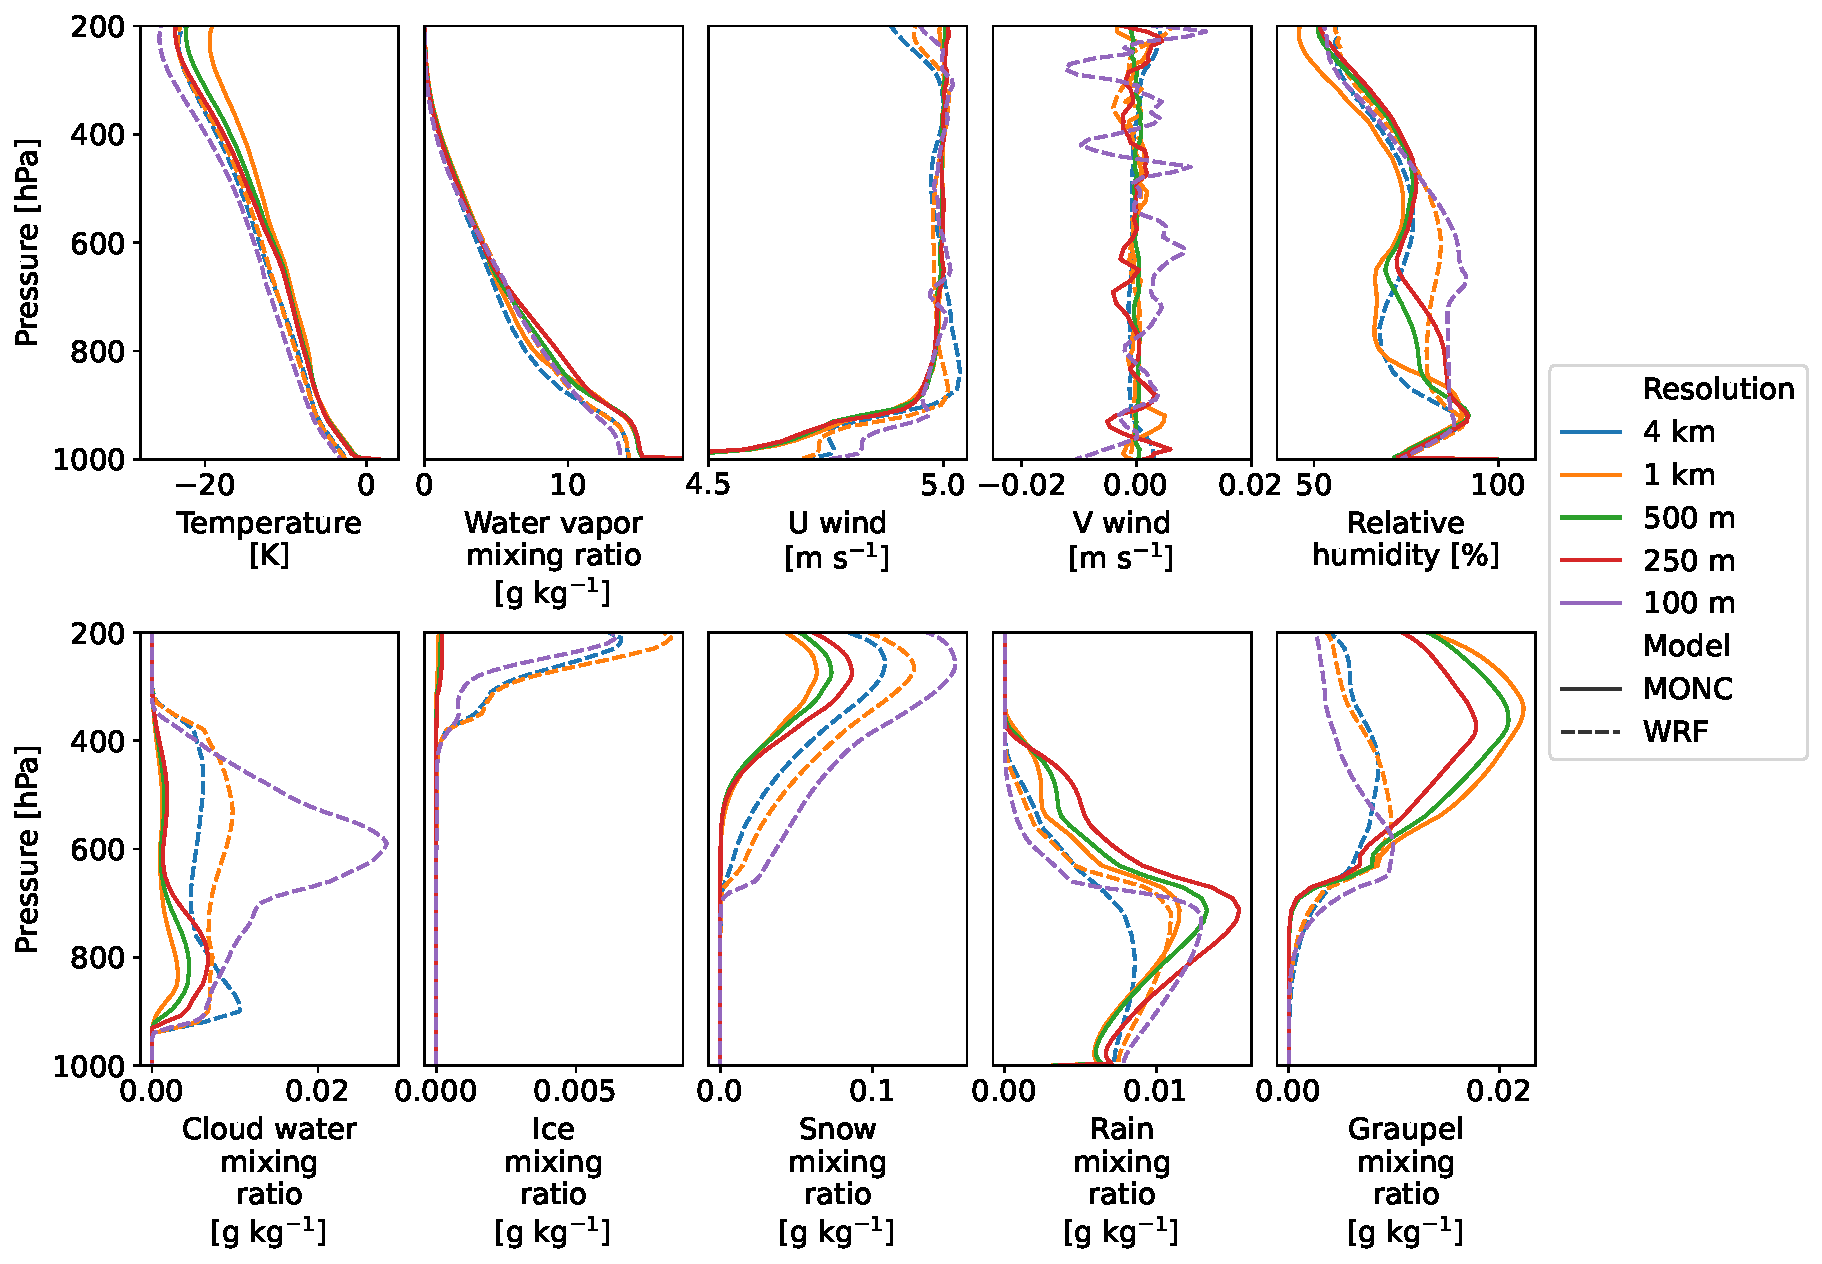
\includegraphics[width=\textwidth]{figures/rce_profiles}
    \caption{Mean profiles for selected variables in the control runs' RCE
    periods, by grid spacing. \todo{Note all plots stop at 200 hPa. Steve: The
    cirrus layer that seems to form at the tropopause should be completely
    irrelevant since it is not affecting radiation (right?) or the convection.
    You can mention in the text that it occurs and isn’t shown.}}
    \label{fig:rce_profiles}
\end{figure}

Hydrometeor profiles, also shown in Figure \ref{fig:rce_profiles}, are sensitive
to resolution. For the WRF runs increasing resolution resulted in more rain
below $\sim$650 hPa and less rain above, increases in cloud droplets and snow
particles, increases in graupel content below $\sim$500 hPa and decreases above,
and mixed changes in ice particle content. The MONC runs showed marginally less
sensitivity, but the character of the changes was broadly the same, with the
exception of rain particles which for MONC runs show an increase with higher
resolution on all levels, and ice particle which show a decrease with higher
resolution on higher levels. Profile shapes are broadly similar between WRF and
MONC, with perhaps the strongest difference in liquid water for which MONC has
significantly more at $\sim$800 hPa and less above $\sim$600 hPa. Graupel and
snow are found at lower heights in WRF than in MONC. We note that the MONC
results are missing the large resolution change between 4 km and 1 km that is
shown in the WRF results. The sharp difference between WRF's cloud droplet
mixing ratio at 1 km compared with 100 m grid spacing just above $\sim$600 hPa
does not have a counterpart in the MONC results. In both models we see an
increase in ice content at cloud top, and in both models there is less graupel
at high resolution, with relative differences varying by height. It is hard to
know whether these microphysics changes are simply a reflection of there being
more moisture in the mean state with resolution, or whether they reflect changes
in the representation of clouds.

\subsection{Convective Organisation}

We tested for convective organisation in by examining the spatial variance of
precipitable water scaled by its spatial mean (in WRF, not shown), and by
examining snapshots of precipitation cross-sections inside the equilibrium
period (in MONC, not shown) and found no evidence of meaningful organisation in
these fixed-radiation setups. Our domain sizes are chosen such that they are
too small for self-aggregation of convection to be expected
\cite{Muller_JAS_2012}.

\subsection{Responses to Perturbations in Temperature}

The responses of the models to perturbations in temperature at 412 hPa (415 hPa
for MONC), and 850 hPa are shown in Figures \ref{fig:tpert_412} and
\ref{fig:tpert_850}, respectively, with results for 500 hPa, 600 hPa, and 730
hPa in Figures \ref{fig:tpert_500}, \ref{fig:tpert_600}, and
\ref{fig:tpert_730}, respectively. In all cases, the moisture and hydrometeor
responses to forcing perturbations are much smaller than the changes in the mean
profiles owing to resolution (Figure \ref{fig:rce_profiles}). WRF and MONC
produce responses of similar amplitude. In the temperature, water vapour mixing
ratio, and relative humidity fields, MONC is more likely to show nonlinearity,
or differences in responses to positive and negative perturbations, than WRF at
1 km or 4 km resolutions, with the strongest example being the temperature
response in the upper troposphere to a temperature perturbation at 850 hPa. The
100 m WRF results also show some apparent non-linearity in their responses. In
the hydrometeor fields, the strongest apparent non-linearity is in the WRF
results at 100 m grid spacing. However, figures \ref{fig:var_T_412} and
\ref{fig:var_T_850} show the $\pm$1 standard deviation range around these mean
responses at 100 m grid spacing. The large range in responses means that the
discrepencies between responses for positive and negative perturbations are less
likely to be caused by non-linearity than by noise in the response signal for
these hydrometeor mixing ratios.

\begin{figure}[pth]
    \noindent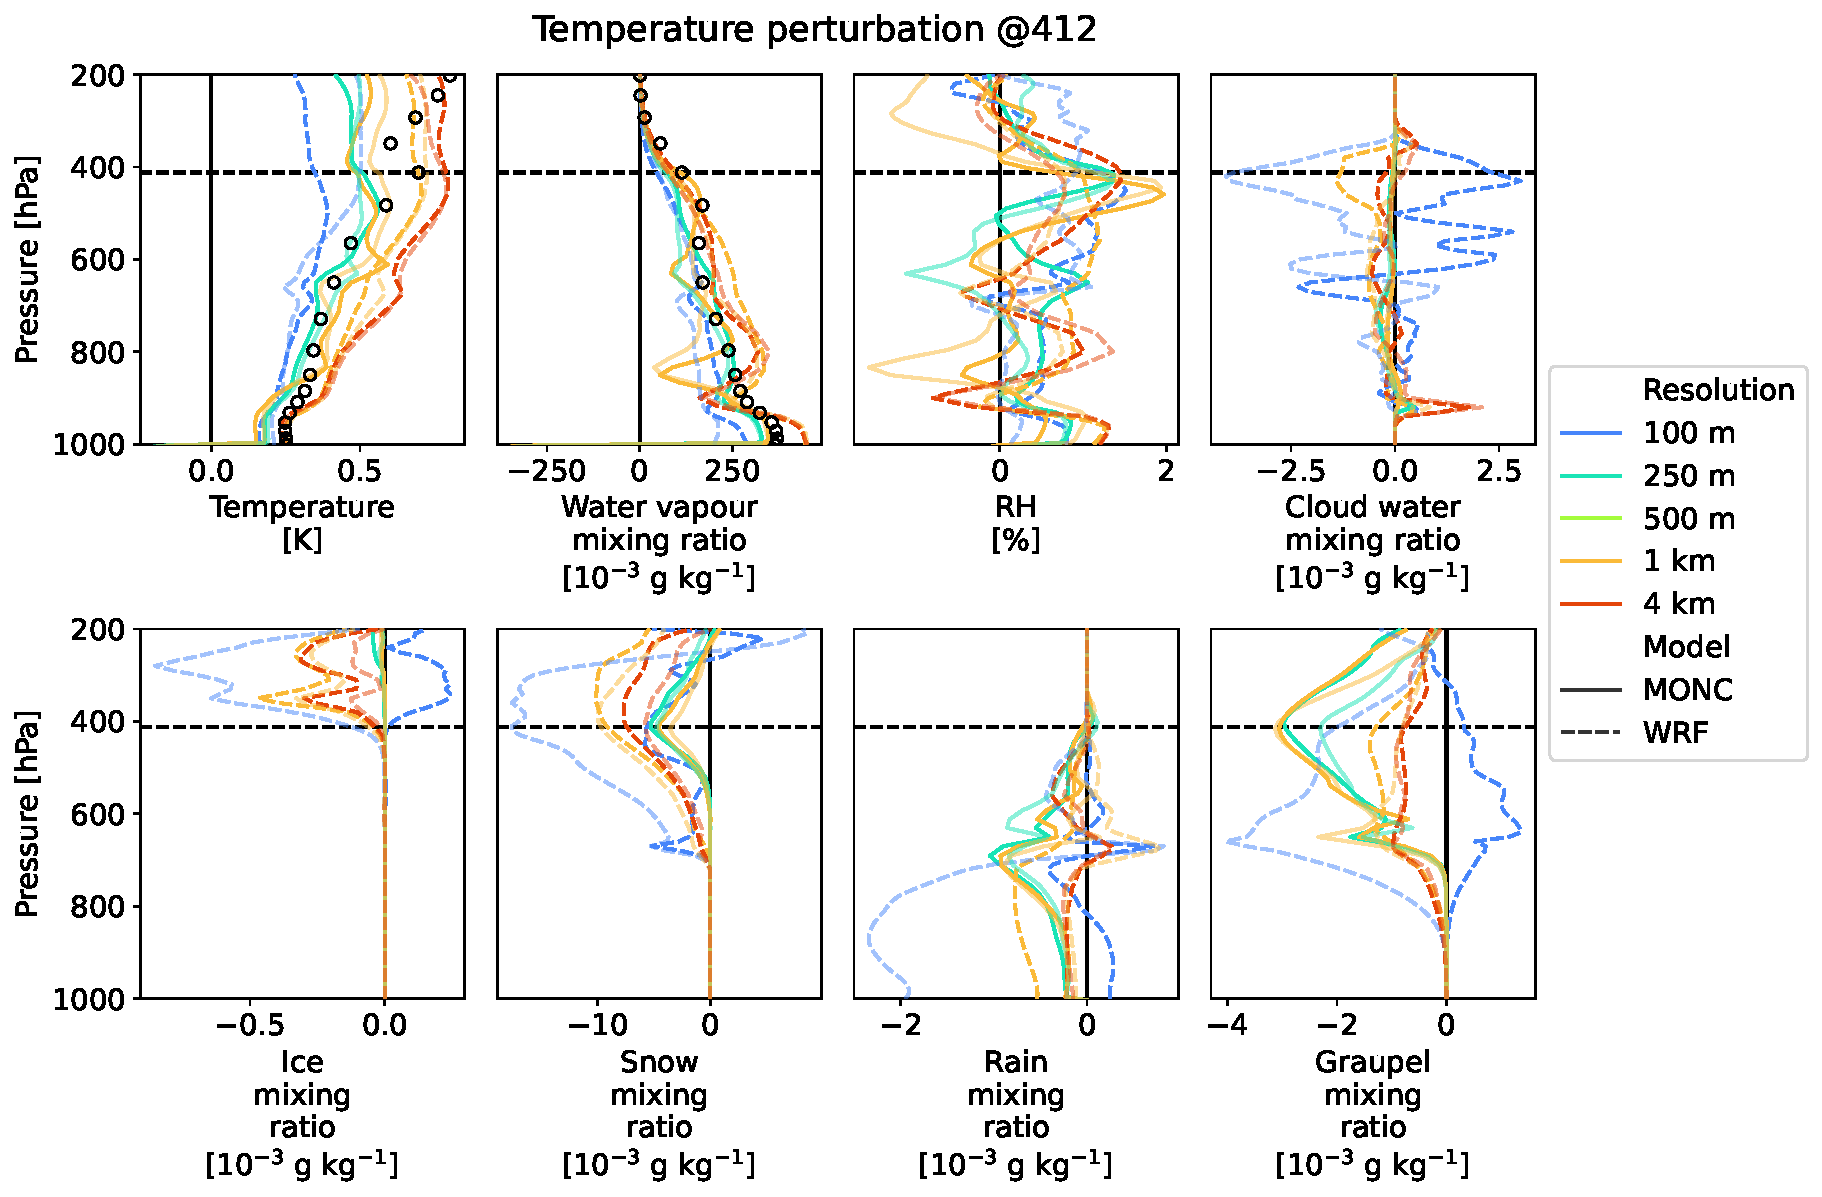
\includegraphics[width=\textwidth]{figures/pert_diffs_T_0.5_@412}
    \caption{Differences in model values by pressure, after a perturbation of
    +0.5 K was introduced in the potential temperature tendency field at 412 hPa
    (415 hPa for MONC). The solid vertical black line shows zero difference. The
    dashed horizontal line shoes the approximate level of maximum perturbation.
    Responses to positive perturbations are shown with opaque lines, while
    responses to negative perturbations are shown with semi-transparent lines.
    Responses to negative perturbations have been multiplied by $-1$ so they
    overlay responses to positive perturbations if the positive and negative
    responses are symmetrical. Black circles show the responses to the same
    perturbation recorded by \citeA{Kuang_JAS_2010}.}
    \label{fig:tpert_412}
\end{figure}

\begin{figure}[pth]
    \noindent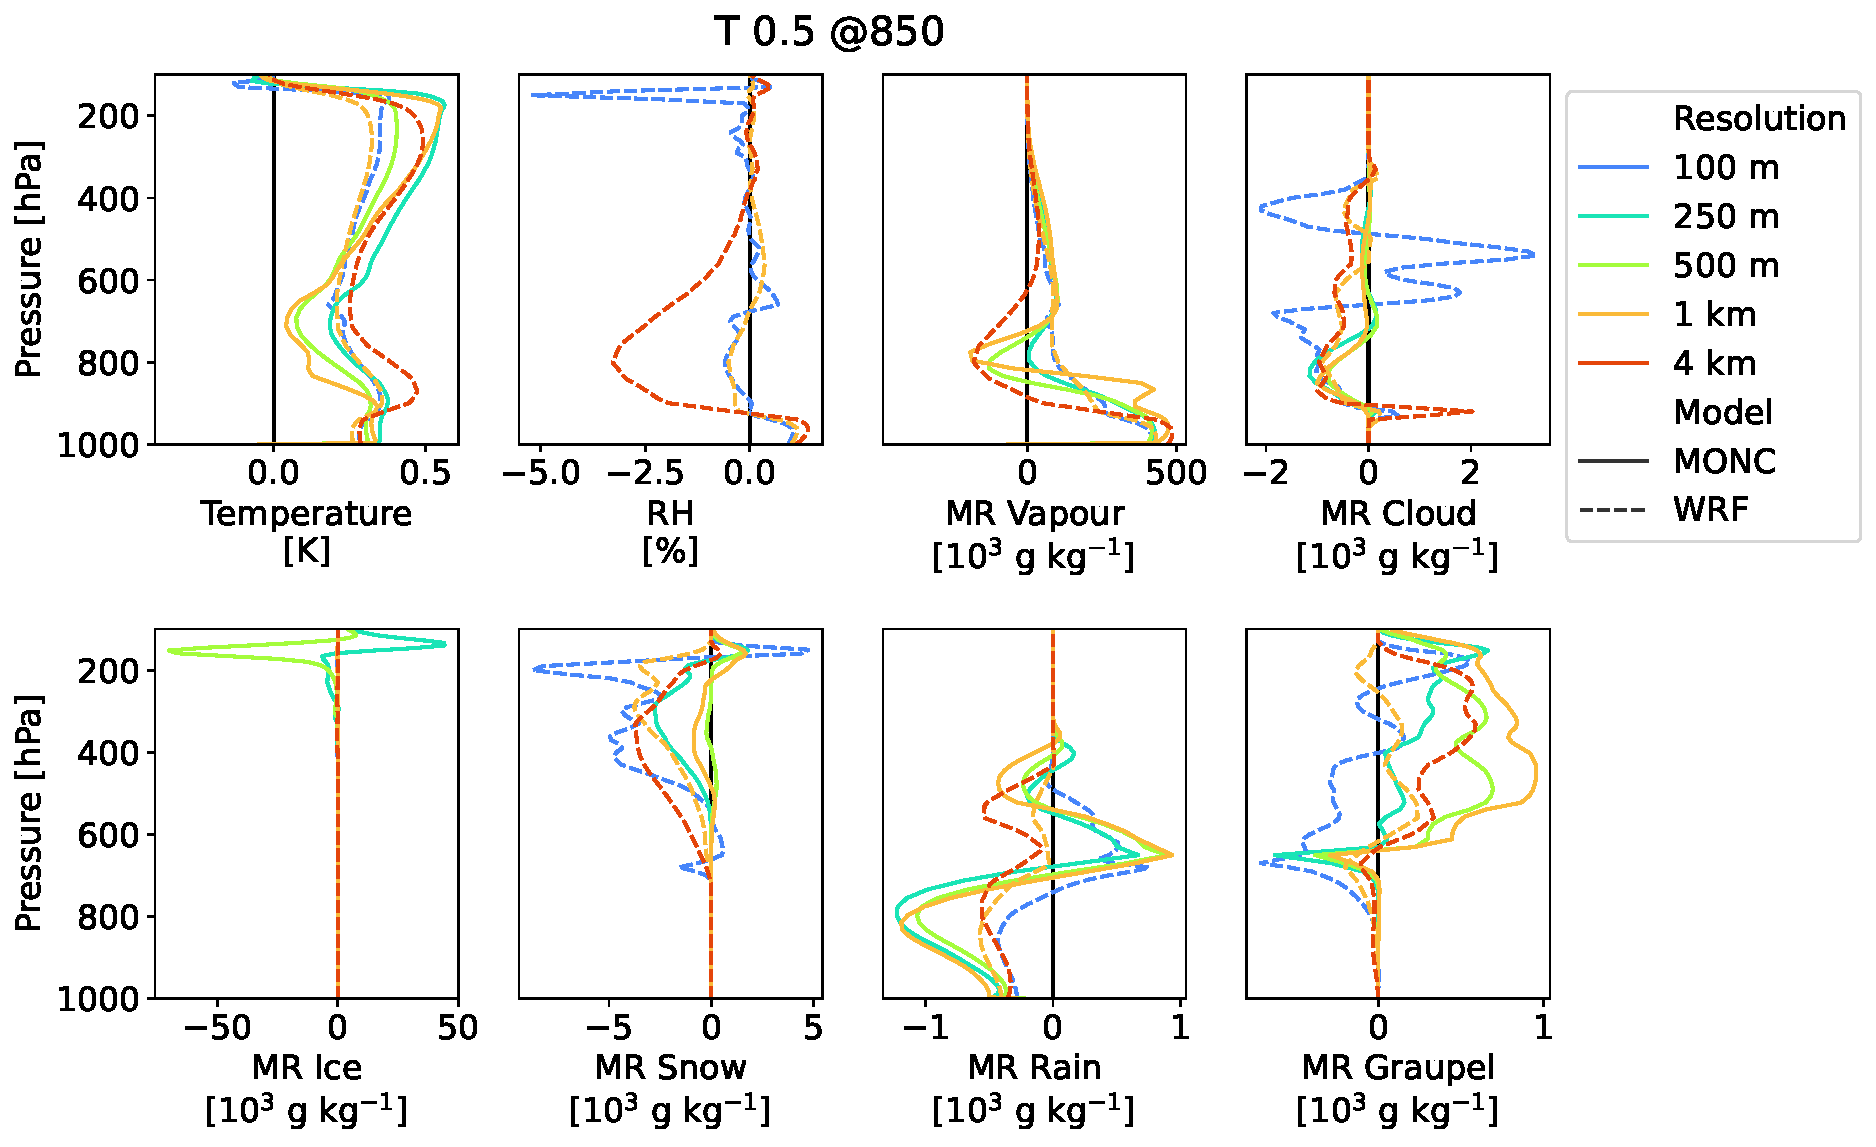
\includegraphics[width=\textwidth]{figures/pert_diffs_T_0.5_@850}
    \caption{As in Figure \ref{fig:tpert_412}, but for a temperature
    perturbation at 850 hPa.}
    \label{fig:tpert_850}
\end{figure}

\subsubsection{Temperature Response}

In response to temperature perturbations, warming tends to increase with height
from the surface to a maximum just below the perturbation level, then decrease
across the perturbation level before once more increasing with height. This
structure is most apparent in the responses to perturbations in the middle
levels (500, 600, 730 hPa), and it is not apparent in the responses for a
perturbation at the low level of 850 hPa. This ``dog leg'' structure is also
often more marked in MONC than in WRF which gives a smoother temperature
response in the vertical. The sub-km resolution runs with MONC also produce
smoother responses than the 1 km runs.

\subsubsection{Moisture Response}

The moisture responses to the temperature perturbations again shows smoother
responses vertically from WRF than from MONC. A temperature perturbation at 412
hPa (415 hPa for MONC) and the perturbation at 850 hPa show the strongest
differences between the various runs. In some cases (WRF at 4 km and MONC at 1
km and 500 m) the 850 hPa perturbation can induce a drying response at and just
above the perturbation level. With WRF, this response becomes a moistening at
finer resolution. With MONC, the drying is a little less marked at 500 m rather
than 1 km, and at 250 m grid spacing the response was zero at this level. For
the temperature perturbation at 850 hPa, moistening in the boundary layer
increases for coarser resolutions in WRF, and to a lesser extent for MONC. A
temperature perturbation at 412 hPa produces a minimum in the moistening in the
WRF runs at around 900 hPa. In MONC there is a similarly pronounced minimum a
little higher at about 850 hPa seen in the 1km run. Similar comments apply for
500 and 600 hPa as for 412 hPa. There is often a small minimum in the moistening
responses around or the perturbation level itself, particularly for
perturbations applied at lower levels (at higher levels a second minimum tends
to appear below the perturbation level). For a temperature perturbation at 730
hPa, the moistening minimum around the application level is pronounced in MONC
and reaches around zero, but it does not produce the drying seen when the
perturbation is applied at 850 hPa. One way to think about the drying with
perturbations at 850 hPa is that the minimum we see consistently just above the
boundary layer combines with the minimum that we often see at or below the
perturbation level.

\subsubsection{Hydrometeor Responses}

We now turn to the responses in hydrometeor content to perturbations in the
temperature field, while keeping in mind the high variability in the 100 m WRF
hydrometeor responses. For the temperature perturbation at 850 hPa in WRF, there
is generally a reduction of rain below the freezing level; MONC shows a stronger
reduction than in WRF below the freezing level but is increased around the
freezing level, which is a feature not seen in the WRF results. With the
exception of a near-surface increase, a reduction in cloud liquid water also
occurs, and this is over a deeper layer in WRF than in MONC. There is also some
reduction to snow and increase in graupel at upper levels. For WRF runs with
temperature perturbations at lower levels, the profiles of liquid water changes
have reductions with minima that are aligned with or just above the perturbation
height. As the perturbation level increases in the WRF runs, a maxima in liquid
water changes appears between the perturbation level and the surface. The 4 km
WRF runs in particular show a sharp increase in cloud water at about 900 hPa
under all temperature perturbations. The responses of hydrometeors in MONC have
a broadly similar character, but some of the amplitudes are quite different.
There are similar amplitudes to WRF for rain, but weaker responses in liquid
water, ice and snow. MONC responded more strongly for graupel, however,
especially in response to perturbations at 412 and 500 hPa. A positive
temperature perturbation generally reduces graupel content with the exception of
some increases at high levels when the perturbation was closer to the surface.
There are some changes in responses with grid length. For the WRF runs the rain
changes tend to increase in magnitude with increasing resolution, while the MONC
responses are more similar. For MONC the liquid water reductions are stronger at
250 m than at 1 km spacings, and for temperature perturbations at lower levels
snow is also more strongly reduced at 250 m than at 1 km grid spacing. The
changes in graupel become weaker with increasing resolution in MONC runs yet
stronger with increasing resolution for WRF runs. 

\subsection{Responses to Perturbations in Moisture}

Figures \ref{fig:var_q_412}, and \ref{fig:var_q_850}

The responses of the models to perturbations in moisture at 412 hPa (415 hPa for
MONC) and 850 hPa are shown in Figures \ref{fig:qpert_412} and
\ref{fig:qpert_850}, respectively, while perturbations for 500 hPa, 600 hPa, and
730 hPa, are shown in Figures \ref{fig:qpert_500}, \ref{fig:qpert_600}, and
\ref{fig:qpert_730}, respectively. Several elements of these results are similar
to the results for temperature perturbations: moisture and hydrometeor responses
to moisture perturbations are smaller than the changes in the mean profiles due
to resolution, WRF and MONC produced responses of similar amplitude, except for
cloud liquid water and ice where the changes in MONC were much smaller, and
again MONC is more likely to show nonlinearity to positive and negative
perturbations in temperature, water vapour and relative humidity fields than WRF
at 1 km and 4 km grid spacings. MONC run responses in relative humidity seem to
be particularly prone to non-linear responses. Similar to the responses to the
temperature perturbations, the strongest apparent non-linearity after moisture
perturbations is in the hydrometeor fields and especially for the 100 m grid
spacing WRF responses, but again there was a large range in responses (Figures
\ref{fig:var_q_412}, and \ref{fig:var_q_850}) meaning that these discrepencies
are likely caused by noise in the response signal.

\begin{figure}[pth]
    \noindent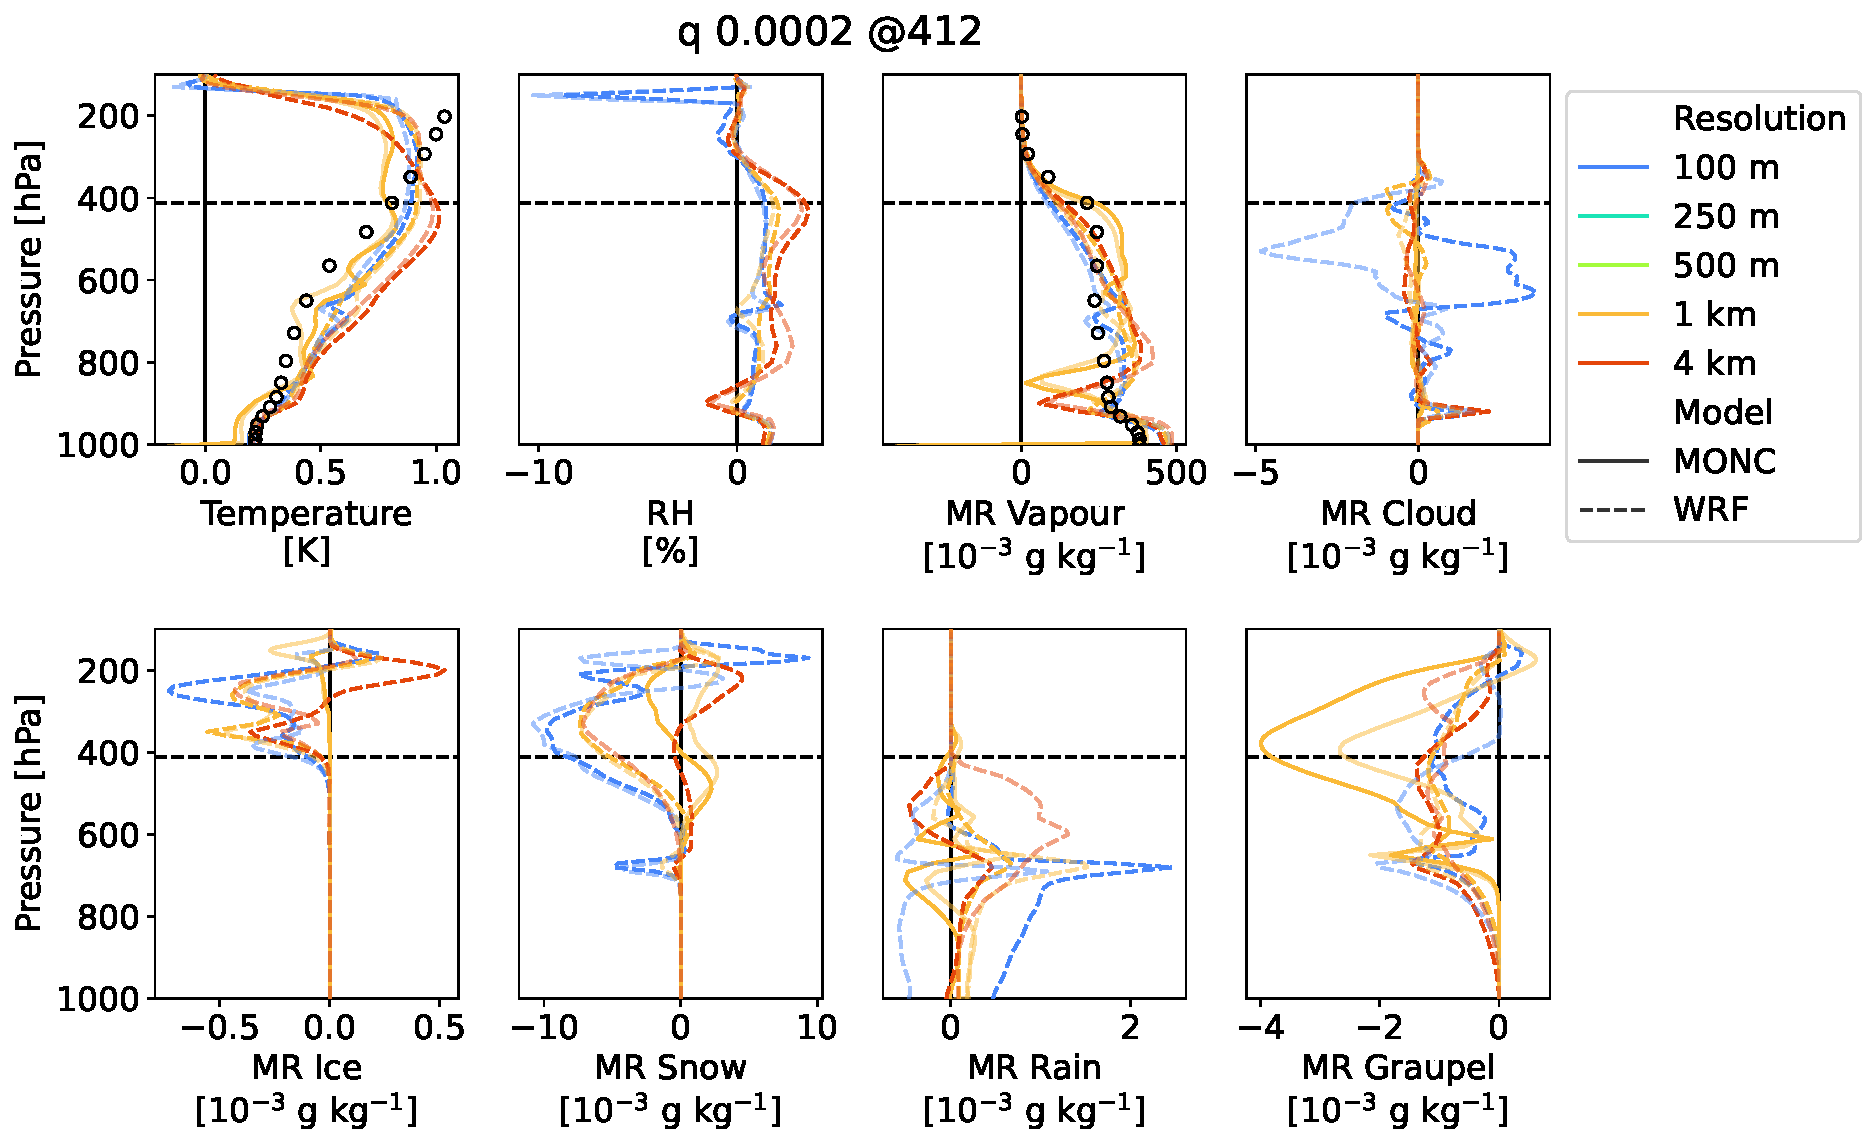
\includegraphics[width=\textwidth]{figures/pert_diffs_q_0.0002_@412}
    \caption{As for Figure \ref{fig:tpert_412}, but for differences in model
    values by pressure, after a perturbation of 0.2 g kg$^{-1}$ was introduced
    in the water vapour mixing ratio tendency field at 412 hPa.}
    \label{fig:qpert_412}
\end{figure}

\begin{figure}[pth]
    \noindent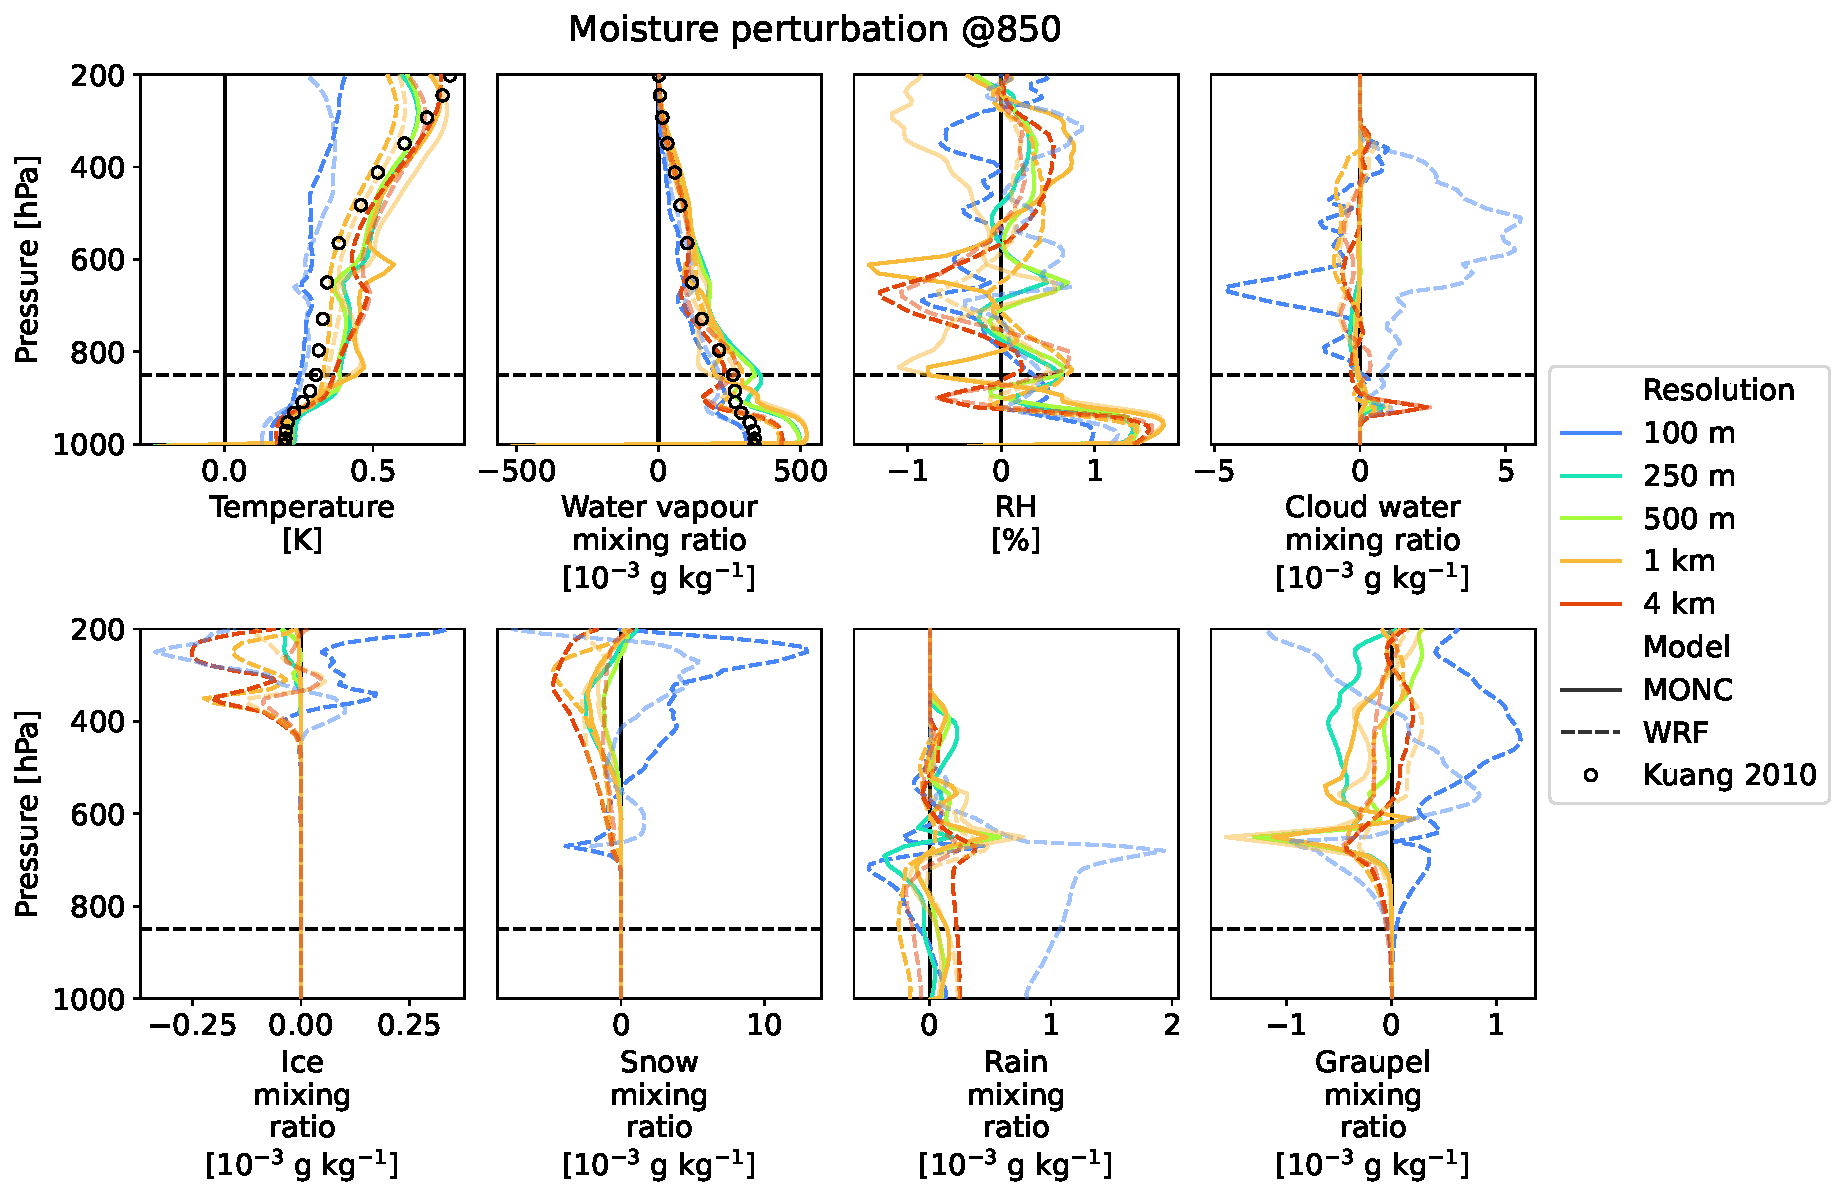
\includegraphics[width=\textwidth]{figures/pert_diffs_q_0.0002_@850}
    \caption{As in Figure \ref{fig:qpert_412}, but for a water vapour mixing
    ratio perturbation at 850 hPa.}
    \label{fig:qpert_850}
\end{figure}

\subsubsection{Temperature Response}

With moisture perturbations, warming in the boundary layer is very consistent
between resolutions in WRF, but the free tropospheric warming is stronger at
coarser resolution and warming is less strong for 100 m grid spacing across the
whole profile. Particularly notable is the increase in warming between 1 km and
4 km grid spacings for a perturbation at 412 hPa. MONC responses show a similar
response below about 600 hPa and above about 850 hPa, but outside this region
the responses for higher resolution runs are stronger than those for 1 km runs.
The boundary layer warming is very consistent between WRF and MONC. The free
tropospheric warming is stronger in MONC for a low-level moisture perturbation
and weaker for an upper-level moisture perturbation.

\subsubsection{Moisture Response}

The response to moisture perturbations in moisture fields in WRF has minima at
around 900 hPa and to a lesser extent around 650 hPa. These minema are modest at
fine grid spacing but at coarse resolution, the lower minimum becomes stronger,
even for perturbations made at upper levels. It does however remain a moistening
response for positive perturbations. Such minima are also present in MONC, the
lower level one being a little higher and much more pronounced than in WRF at
the same grid spacings, and the MONC responses also remaining moistening for
positive perturbations.

\subsubsection{Hydrometeor Responses}

There are non-linearities in the hydrometeor responses, with the most obvious
case that of rain mixing ratios. With some exceptions, increased moisture
tendency shows a small reduction in cloud liquid water across the whole profile
but an increase close to the surface, reductions in ice in the high troposphere,
and reductions in snow above the perturbation level. Graupel is consistently
strongly reduced around 600 hPa but there are responses with opposite signs in
the upper levels. The responses of hydrometeors in MONC are generally weaker
than WRF for liquid water, ice and snow. MONC responds more strongly for
graupel, however, especially in response to higher level perturbations where
non-linearities are evident.

\section{Conclusions}
\label{sec:conclusions}

\begin{itemize}
\item \todo{Hydrometeor responses show much more noise than temperature, water vapour mixing ratio, and relative humidity responses.}
\item \todo{Steve: We need to think about what the main outcomes are (say, our
three bullets).  The conclusion that I think would be most interesting to the
broader community is the resolution needed for each model to approach apparent
convergence of these time-averaged responses (noting that it isn’t a rigorous
convergence test due to computational limitations).  The result suggests that
for most models, to simulate convectively coupled dynamics correctly will likely
require better resolution than is currently used in e.g. DYAMOND. Another
conclusion is that tangent linear responses become relatively similar across
several LES models once this resolution is reached, and so can be used as ground
truth for testing GCM schemes.  Would be good to work through the results to see
how confident we are in such findings, how important each one is, and if there
are other key findings (another one you mention is the relative robustness of
different types of response e.g. T vs q at different levels).}
\end{itemize}

%% Enter Figures and Tables near as possible to where they are first mentioned:
%
% DO NOT USE \psfrag or \subfigure commands.
%
% Figure captions go below the figure.
% Table titles go above tables;  other caption information
%  should be placed in last line of the table, using
% \multicolumn2l{$^a$ This is a table note.}

% \begin{figure}
% \noindent\includegraphics[width=\textwidth]{anothersample.png}
% \caption{caption}
% \label{pngfiguresample}
% \end{figure}

% Acronyms
%  \begin{acronyms}
%  \acro{Acronym}
%  Definition here
%  \acro{EMOS}
%  Ensemble model output statistics
%  \acro{ECMWF}
%  Centre for Medium-Range Weather Forecasts
%  \end{acronyms}

\section{Open Research}

% AGU requires an Availability Statement for the underlying data needed to
% understand, evaluate, and build upon the reported research at the time of peer
% review and publication.

% Authors should include an Availability Statement for the software that has a
% significant impact on the research. Details and templates are in the
% Availability Statement section of the Data and Software for Authors Guidance:
% \url{https://www.agu.org/Publish-with-AGU/Publish/Author-Resources/Data-and-Software-for-Authors#availability}

% It is important to cite individual datasets in this section and, and they must
% be included in your bibliography. Please use the type field in your bibtex file
% to specify the type of data cited. Options include [Dataset], [Software],
% [ComputationalNotebook], [Collection].
% Example:
%
%@misc{https://doi.org/10.7283/633e-1497,
%  doi = {10.7283/633E-1497},
%  url = {https://www.unavco.org/data/doi/10.7283/633E-1497},
%  author = {de Zeeuw-van Dalfsen, Elske and Sleeman, Reinoud},
%  title = {KNMI Dutch Antilles GPS Network - SAB1-St_Johns_Saba_NA P.S.},
%  publisher = {UNAVCO, Inc.},
%  year = {2019},
%  type = {dataset}
%}

\bibliography{library}

\newpage
\section*{Appendix}
\setcounter{figure}{0}
\renewcommand{\thefigure}{A\arabic{figure}}

\begin{figure}[pth]
    \noindent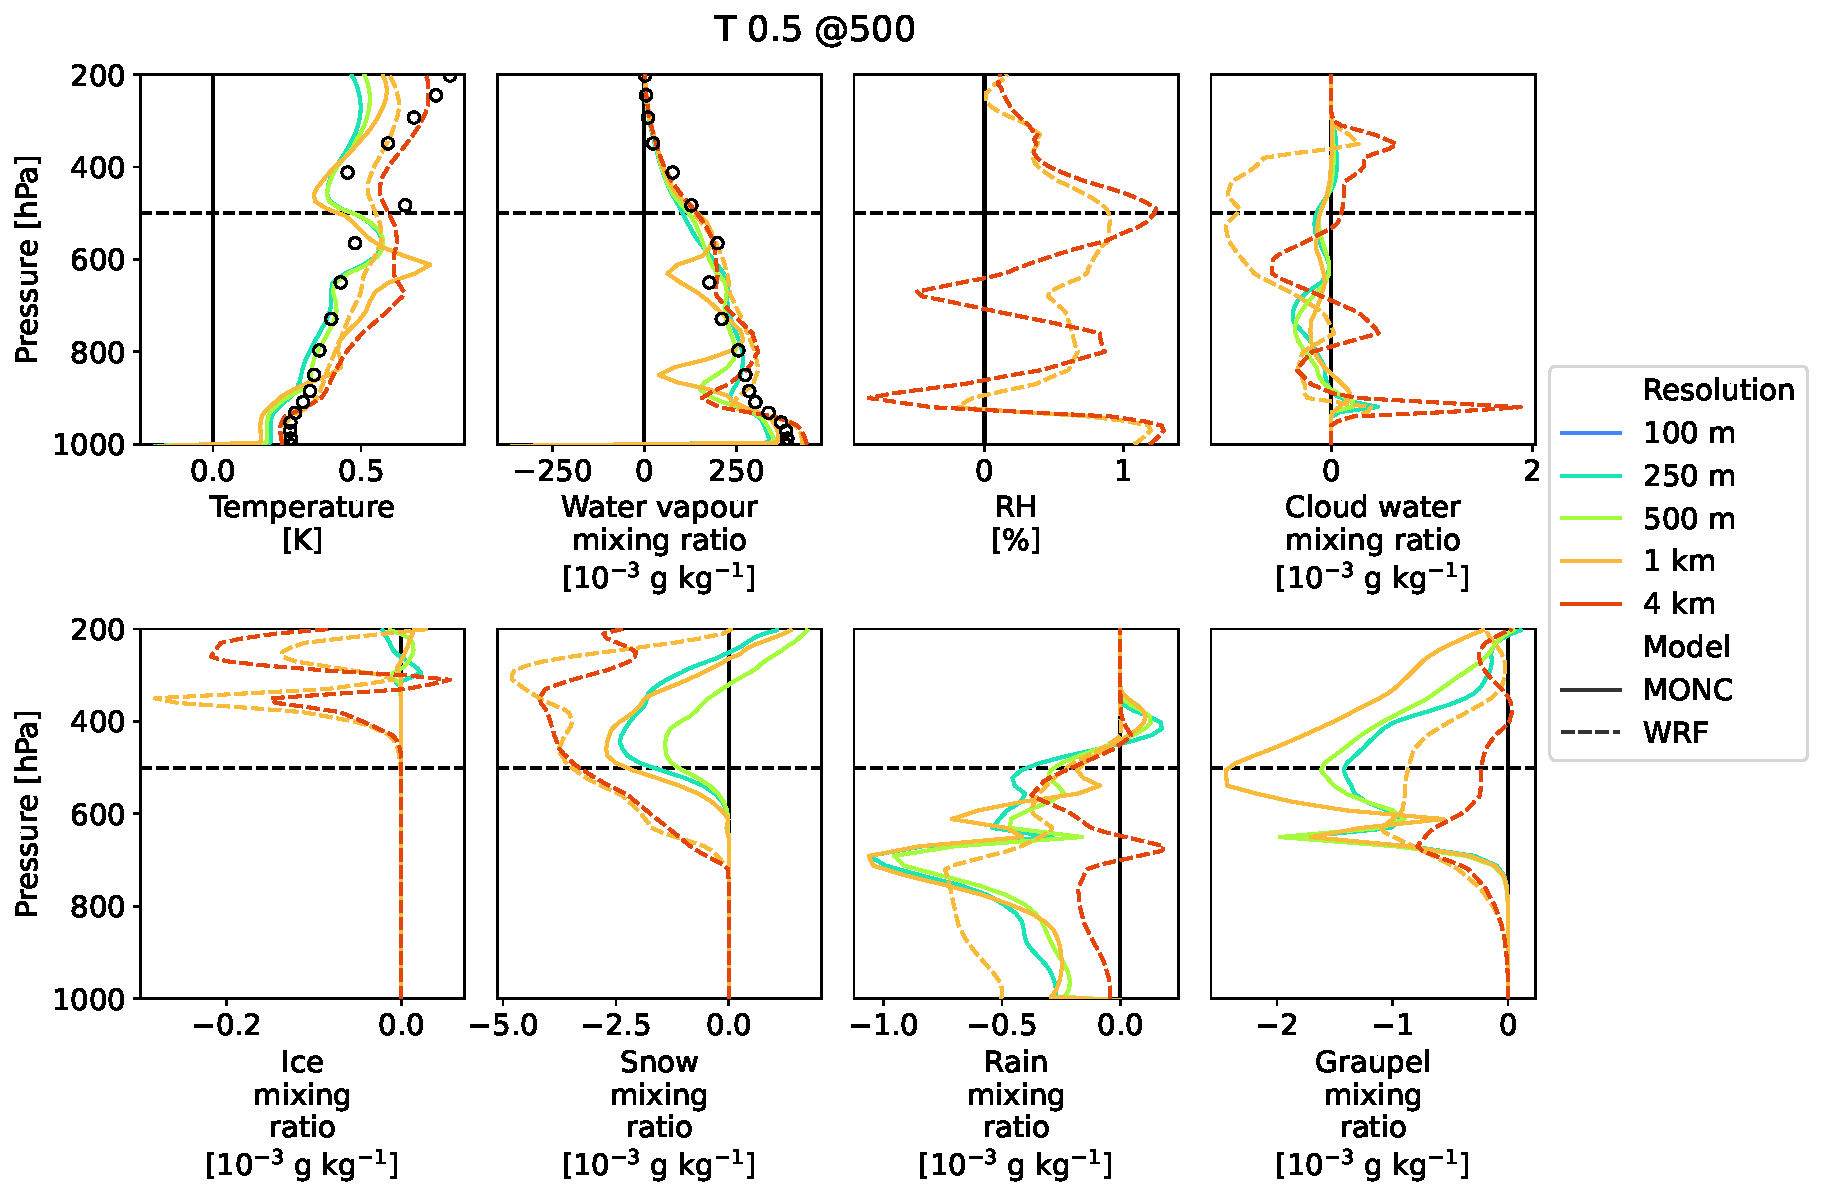
\includegraphics[width=\textwidth]{figures/pert_diffs_T_0.5_@500}
    \caption{As in Figure \ref{fig:tpert_412}, but for a temperature
    perturbation at 500 hPa, and with black circles showing the responses of
    \citeA{Kuang_JAS_2010} to a temperature perturbation at 483 hPa.}
    \label{fig:tpert_500}
\end{figure}

\begin{figure}[pth]
    \noindent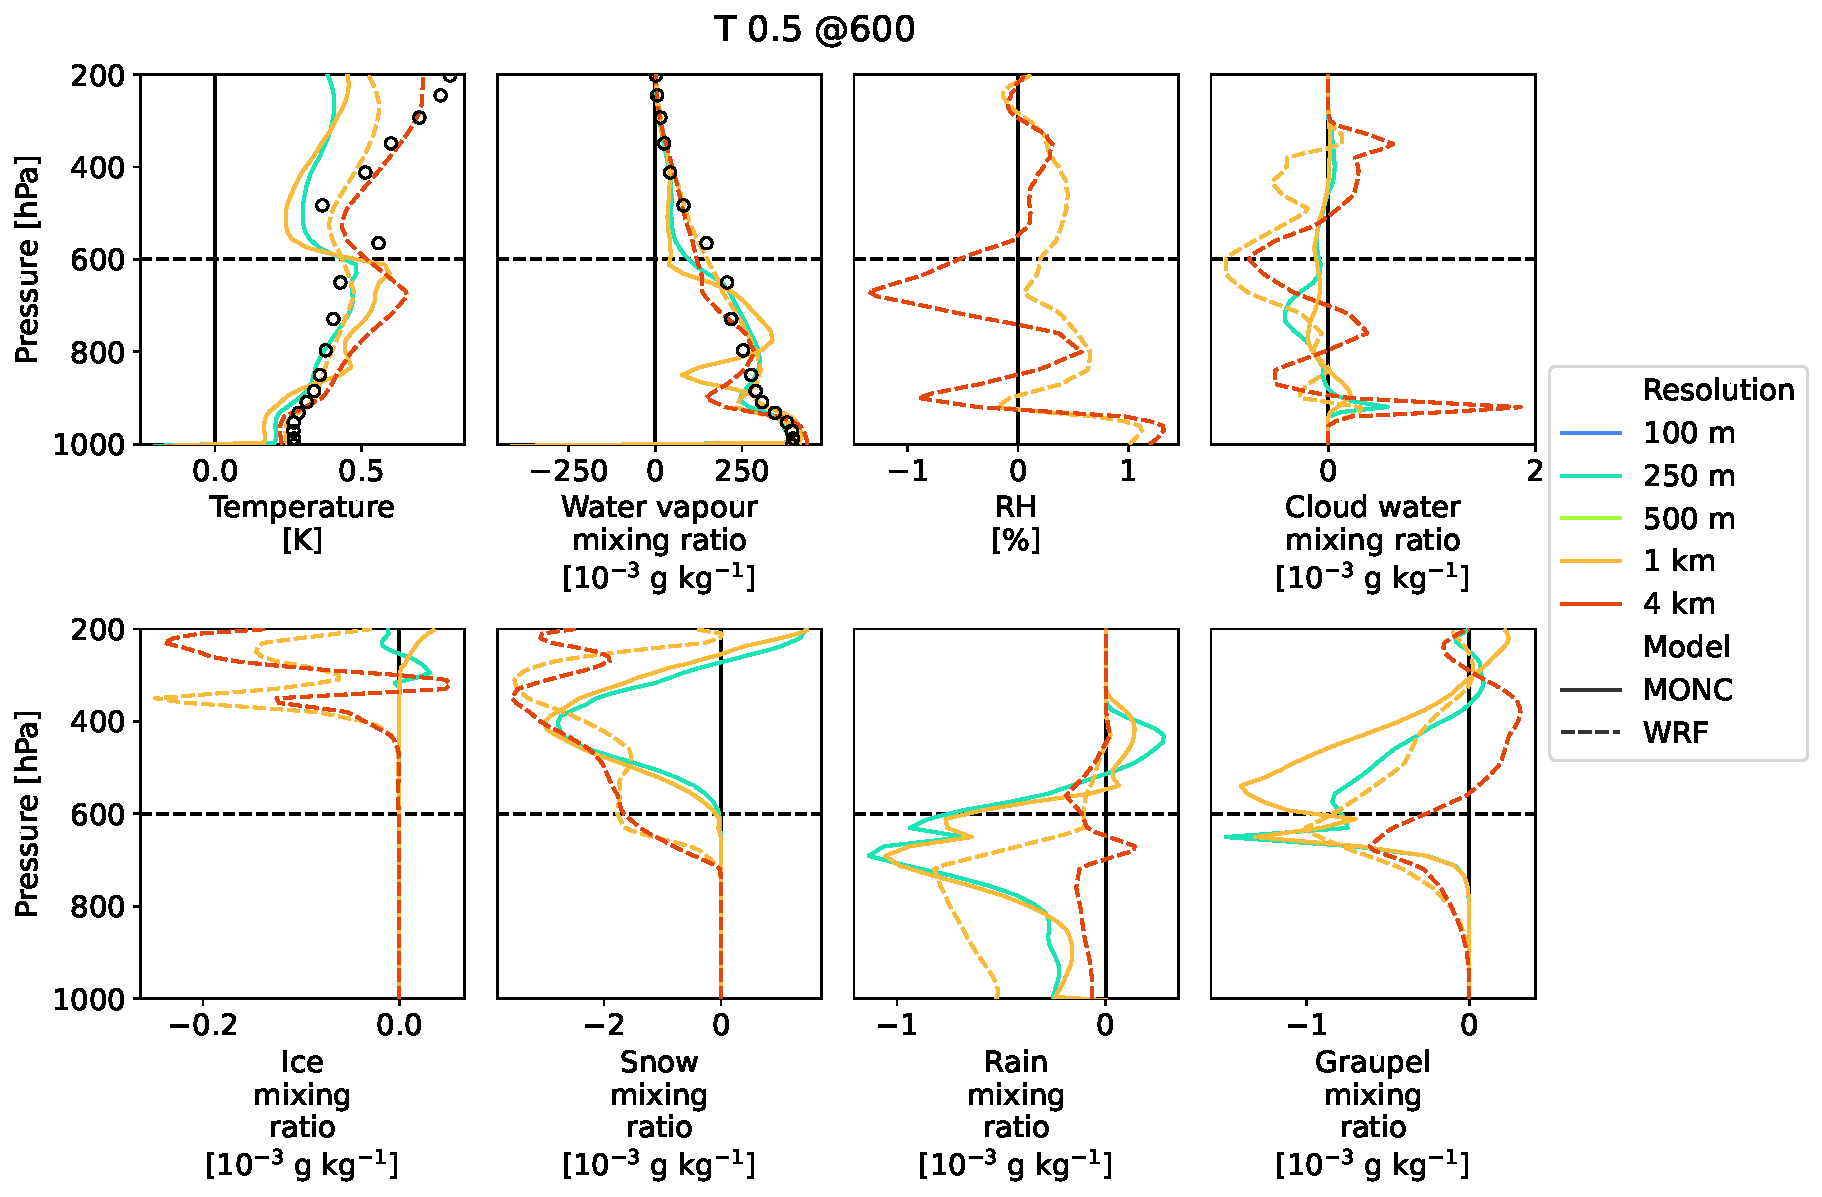
\includegraphics[width=\textwidth]{figures/pert_diffs_T_0.5_@600}
    \caption{As in Figure \ref{fig:tpert_412}, but for a temperature
    perturbation at 600 hPa, and with black circles showing the responses of
    \citeA{Kuang_JAS_2010} to a temperature perturbation at 565 hPa.}
    \label{fig:tpert_600}
\end{figure}

\begin{figure}[pth]
    \noindent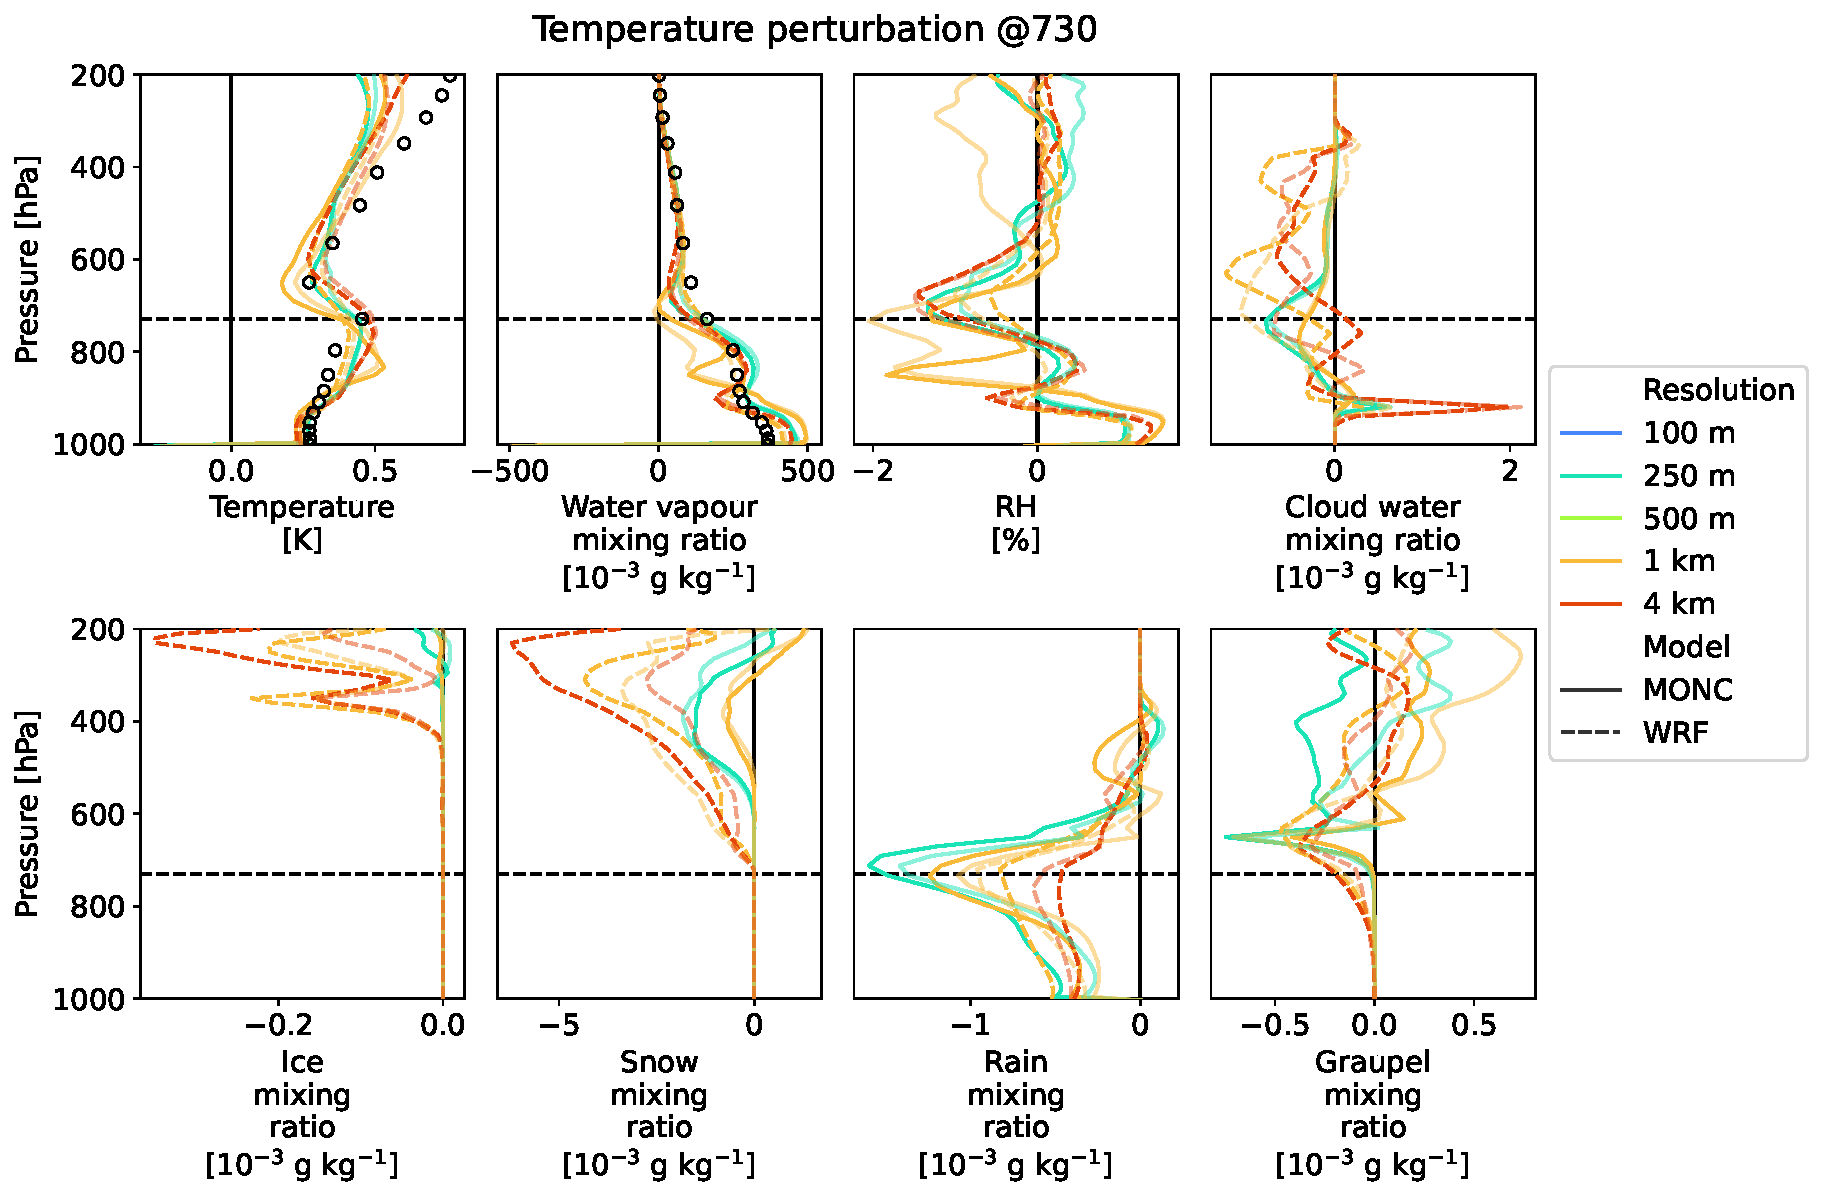
\includegraphics[width=\textwidth]{figures/pert_diffs_T_0.5_@730}
    \caption{As in Figure \ref{fig:tpert_412}, but for a temperature
    perturbation at 730 hPa, and with black circles showing the responses of
    \citeA{Kuang_JAS_2010} to a temperature perturbation at 729 hPa.}
    \label{fig:tpert_730}
\end{figure}

\begin{figure}[pth]
    \noindent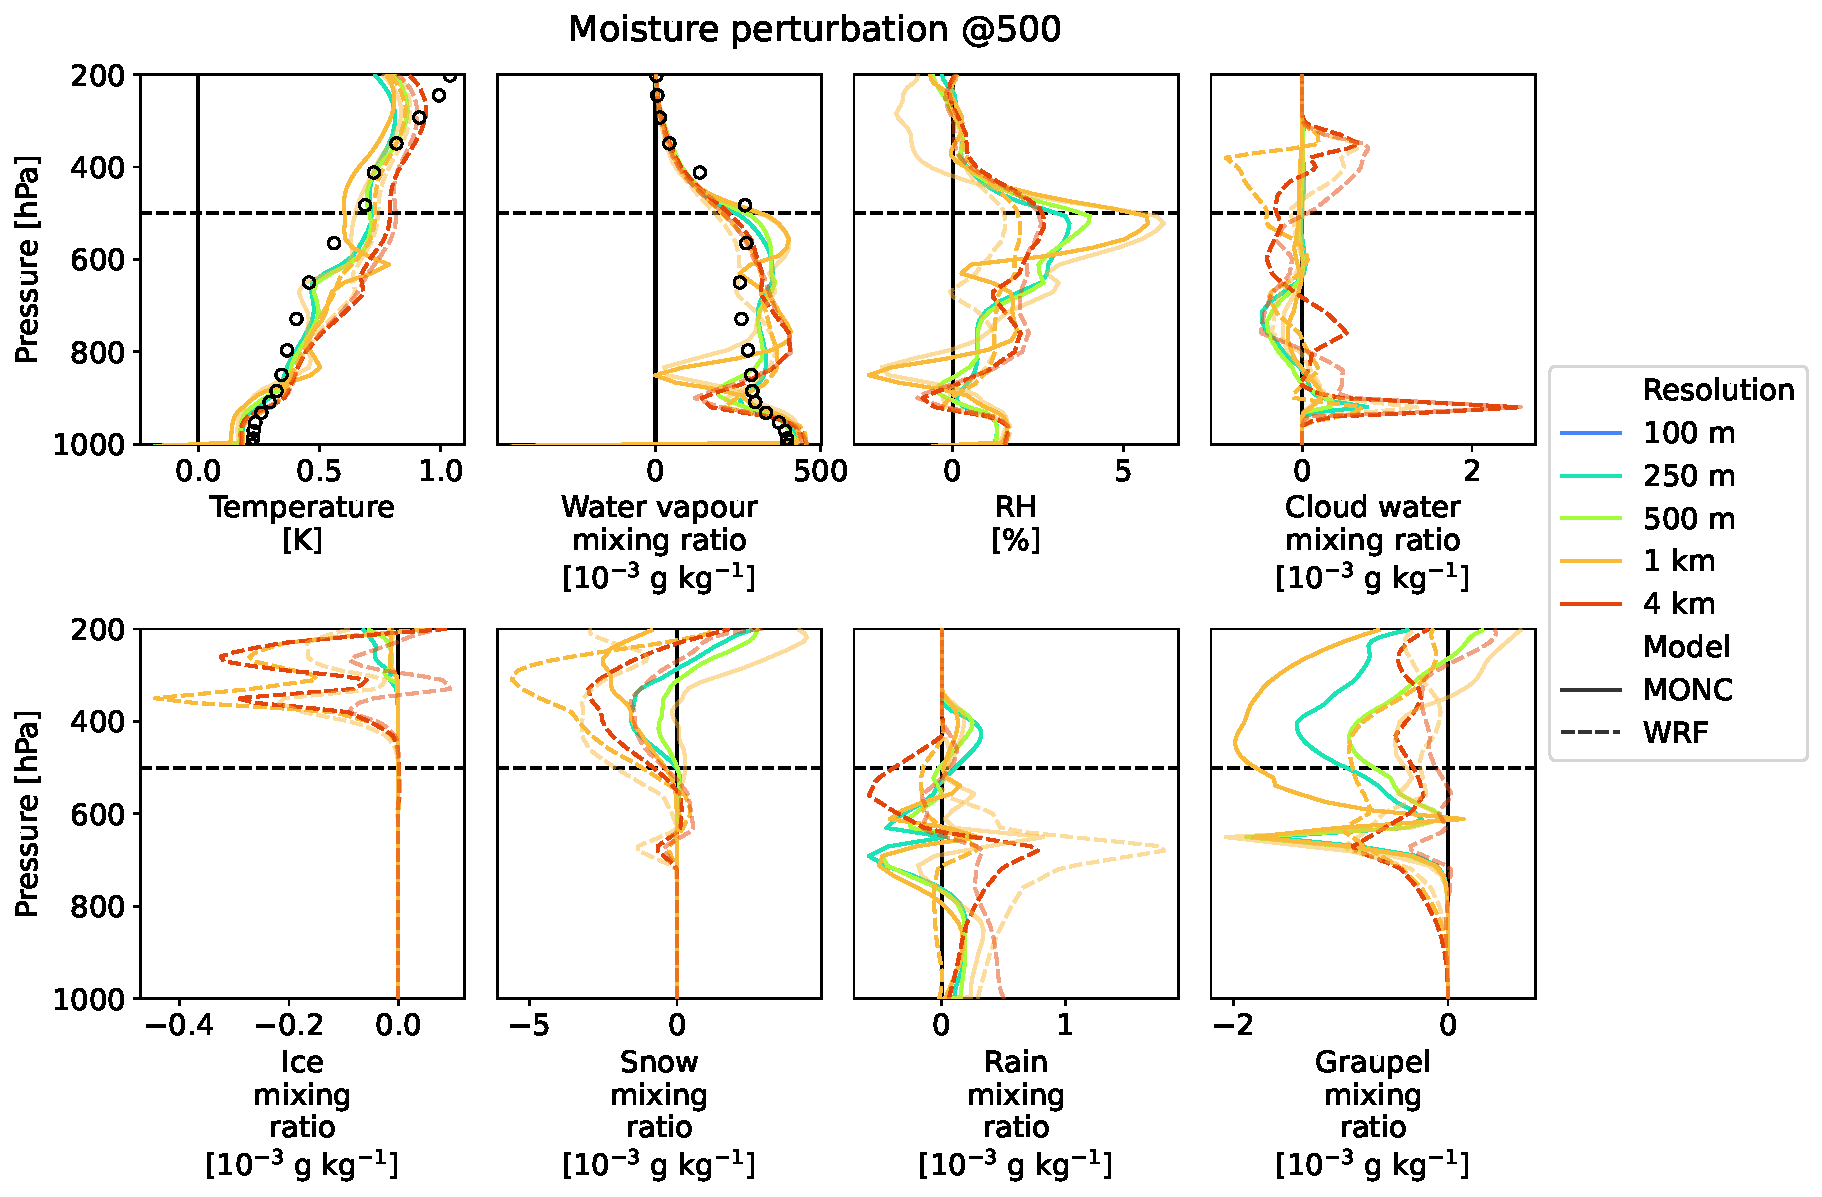
\includegraphics[width=\textwidth]{figures/pert_diffs_q_0.0002_@500}
    \caption{As in Figure \ref{fig:qpert_412}, but for a water vapour mixing
    ratio perturbation at 500 hPa, and with black circles showing the responses
    of \citeA{Kuang_JAS_2010} to a specific humidity perturbation at 483
    hPa.}
    \label{fig:qpert_500}
\end{figure}

\begin{figure}[pth]
    \noindent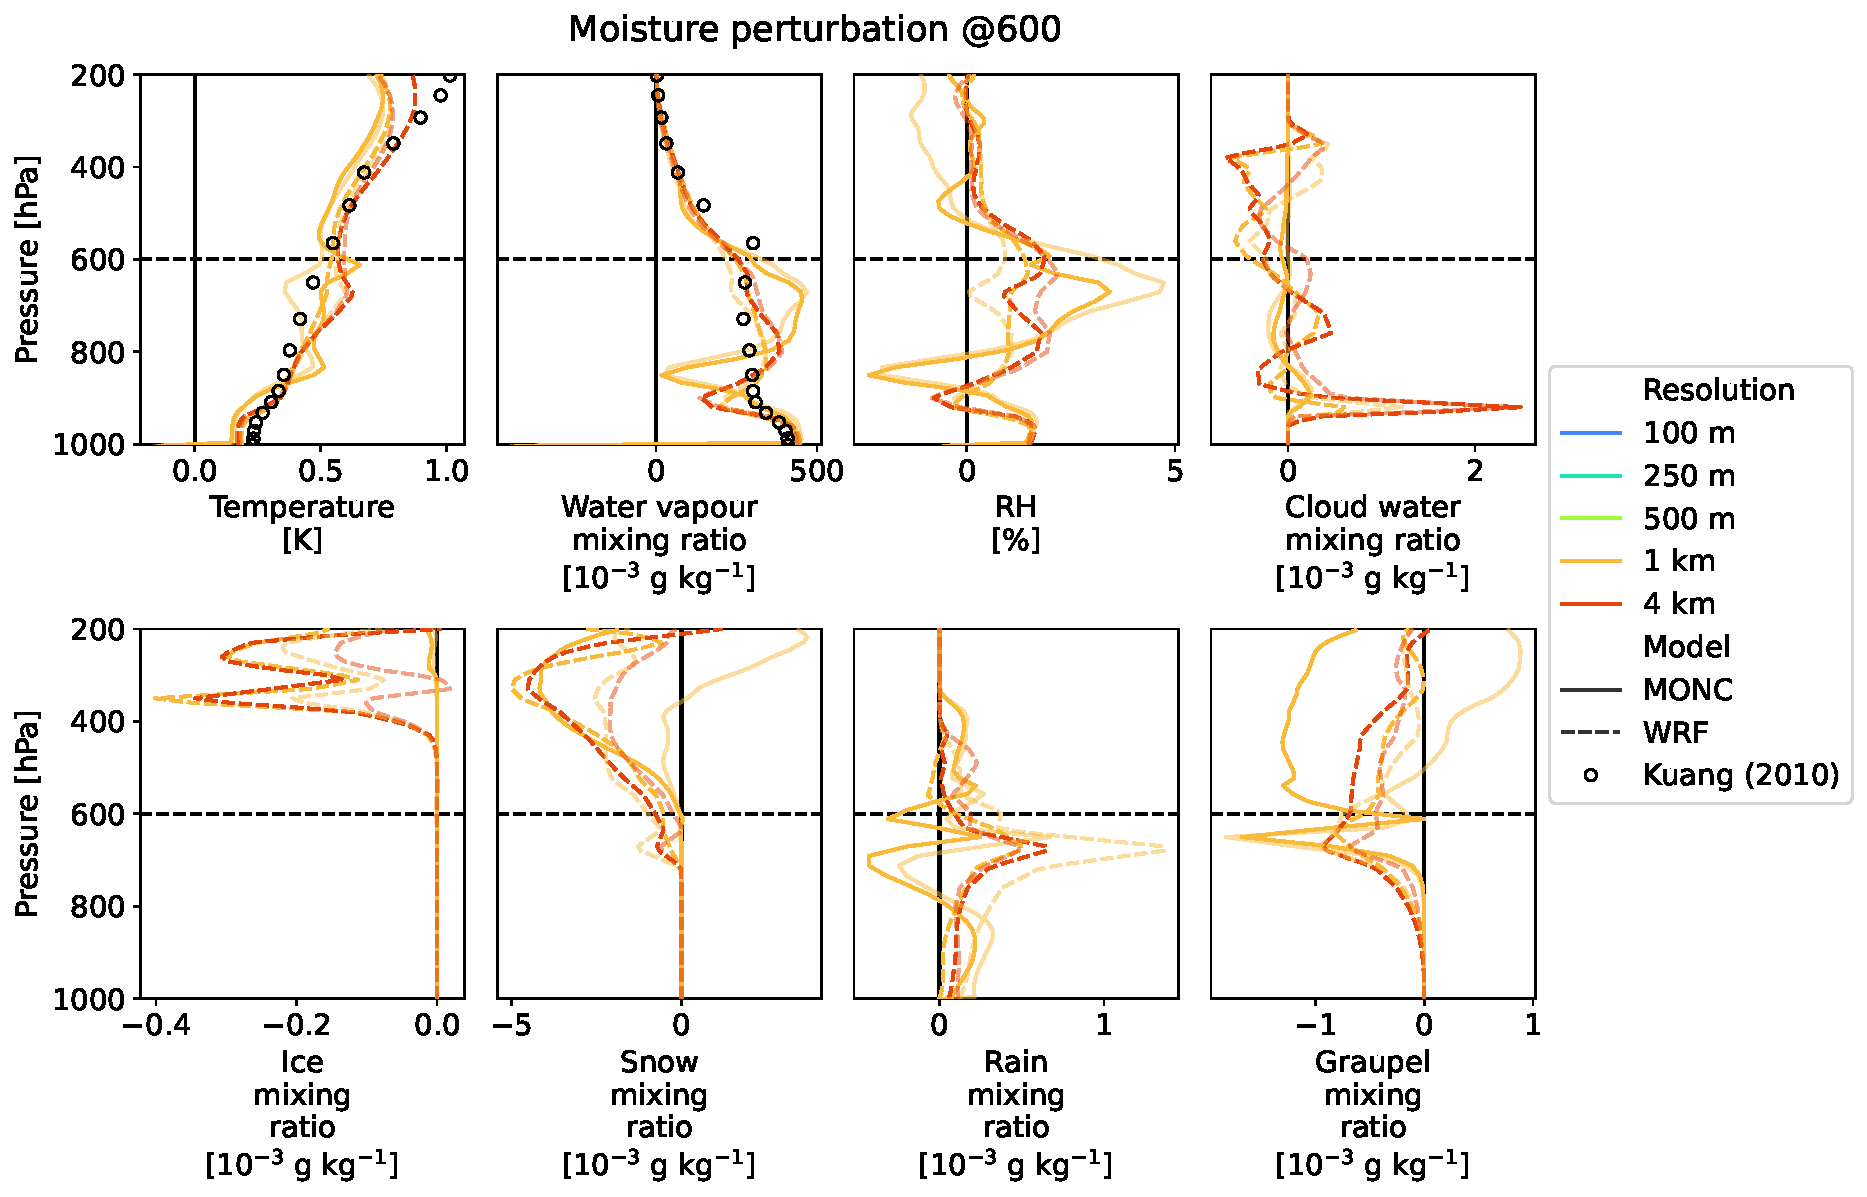
\includegraphics[width=\textwidth]{figures/pert_diffs_q_0.0002_@600}
    \caption{As in Figure \ref{fig:qpert_412}, but for a perturbation at 600
    hPa, and with black circles showing the responses of \citeA{Kuang_JAS_2010}
    to a specific humidity perturbation at 565 hPa.}
    \label{fig:qpert_600}
\end{figure}

\begin{figure}[pth]
    \noindent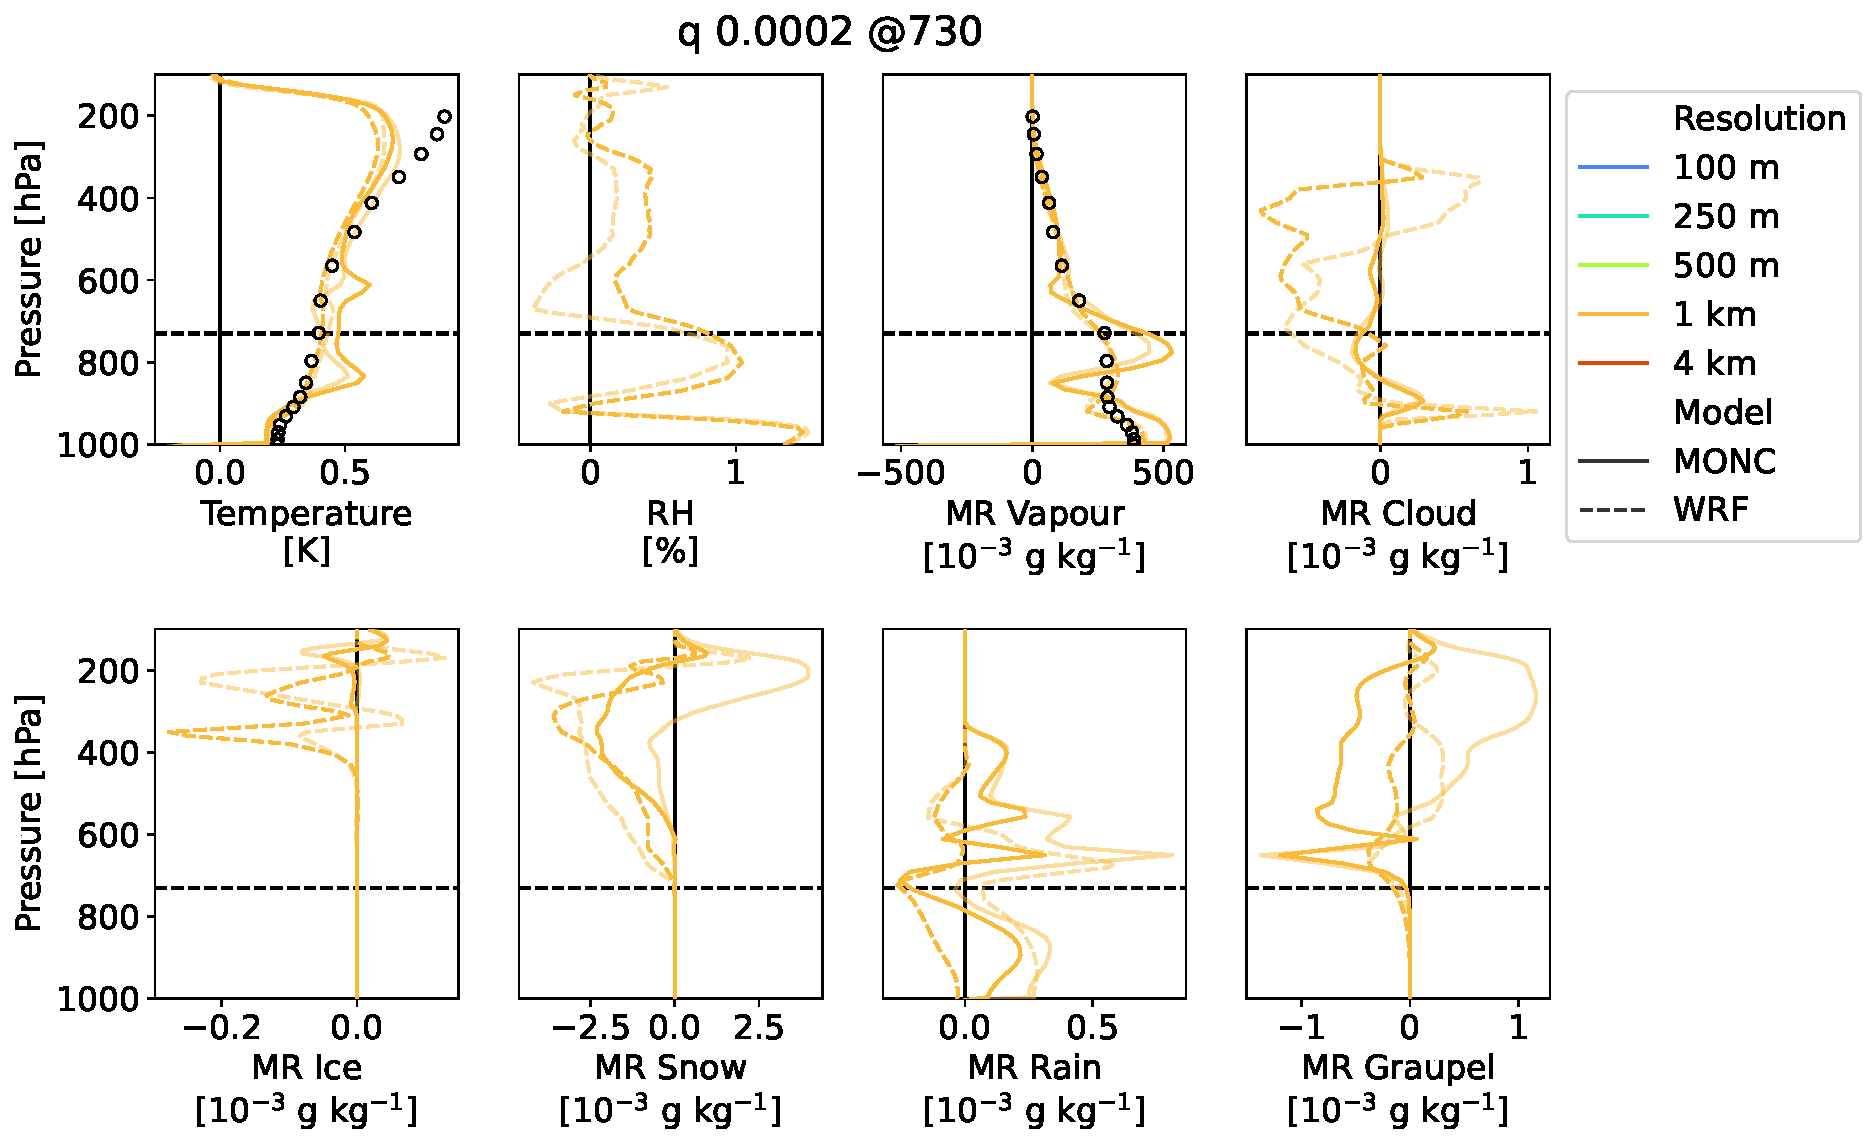
\includegraphics[width=\textwidth]{figures/pert_diffs_q_0.0002_@730}
    \caption{As in Figure \ref{fig:qpert_412}, but for a perturbation at 730
    hPa, and with black circles showing the responses of \citeA{Kuang_JAS_2010}
    to a specific humidity perturbation at 729 hPa.}
    \label{fig:qpert_730}
\end{figure}

\begin{figure}[pth]
    \noindent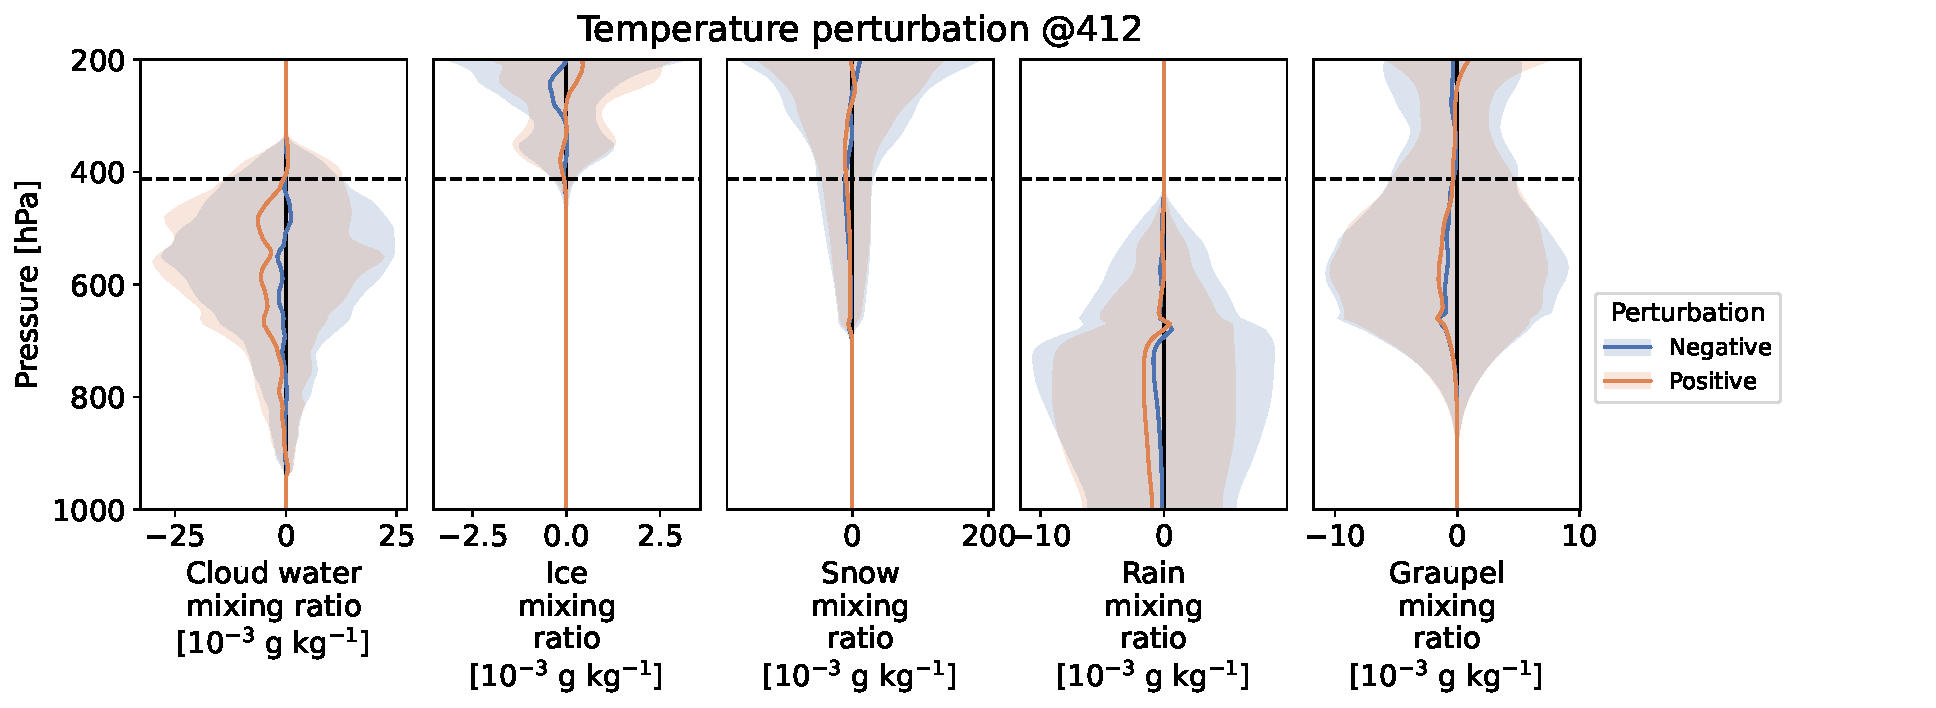
\includegraphics[width=\textwidth]{figures/pert_var_T_0.5_@412}
    \caption{Mean responses (solid line) and the $\pm$ 1 standard deviation range (shaded) for a temperature perturbation of $\pm$0.5 K at 412 hPa in the WRF runs at 100 m grid spacing. The solid vertical line shows zero response, the dashed horizontal line shows the level of maximum perturbation.}
    \label{fig:var_T_412}
\end{figure}

\begin{figure}[pth]
    \noindent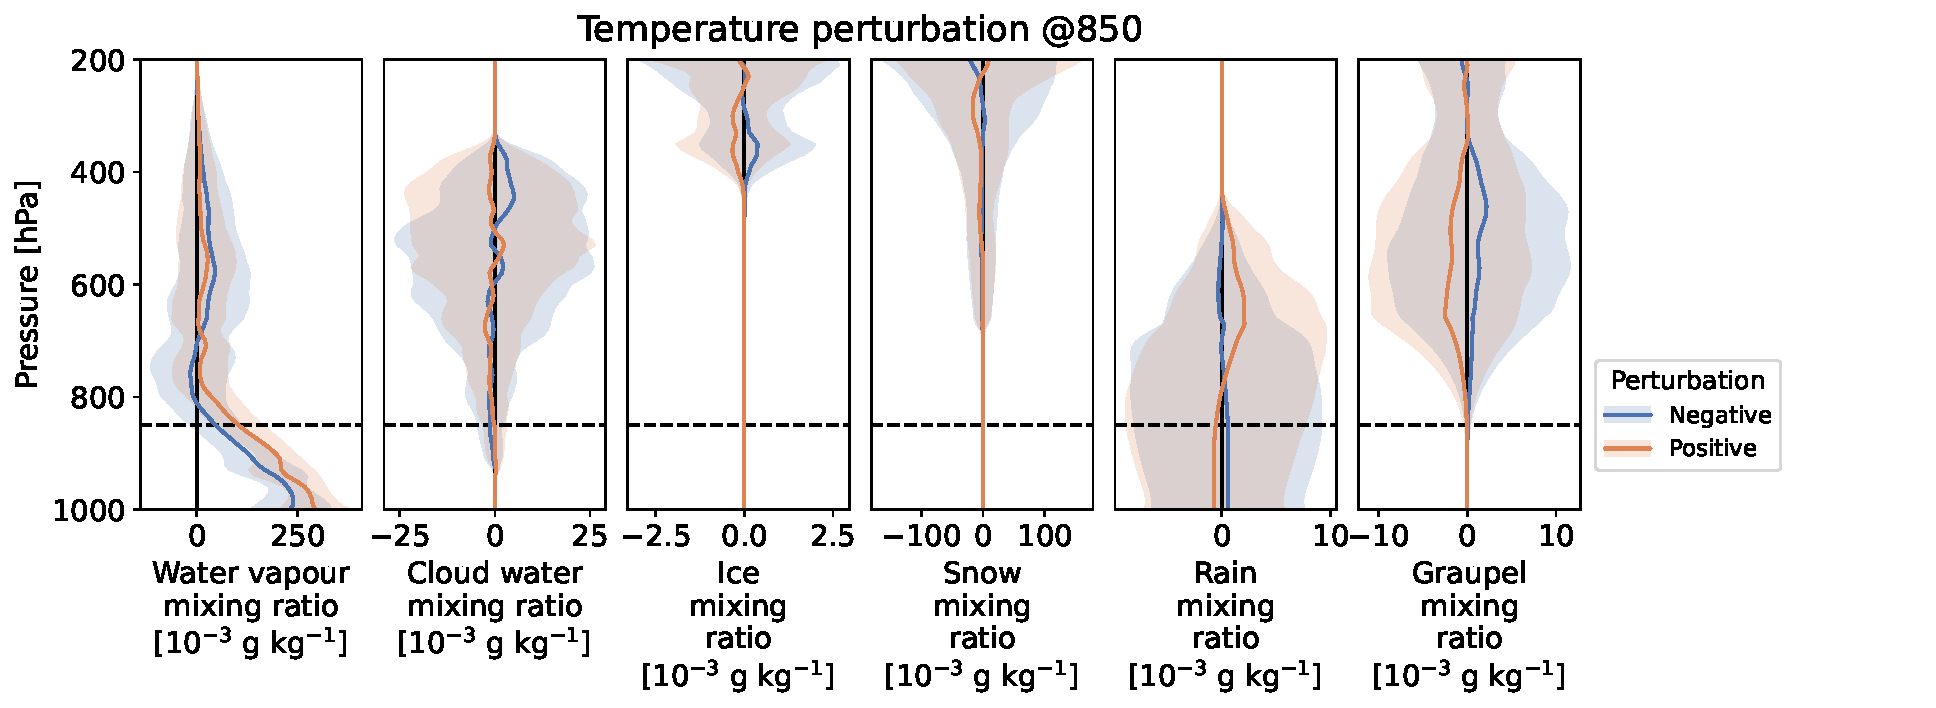
\includegraphics[width=\textwidth]{figures/pert_var_T_0.5_@850}
    \caption{As in Figure \ref{fig:var_T_412} but for a temperature perturbation at 850 hPa.}
    \label{fig:var_T_850}
\end{figure}

\begin{figure}[pth]
    \noindent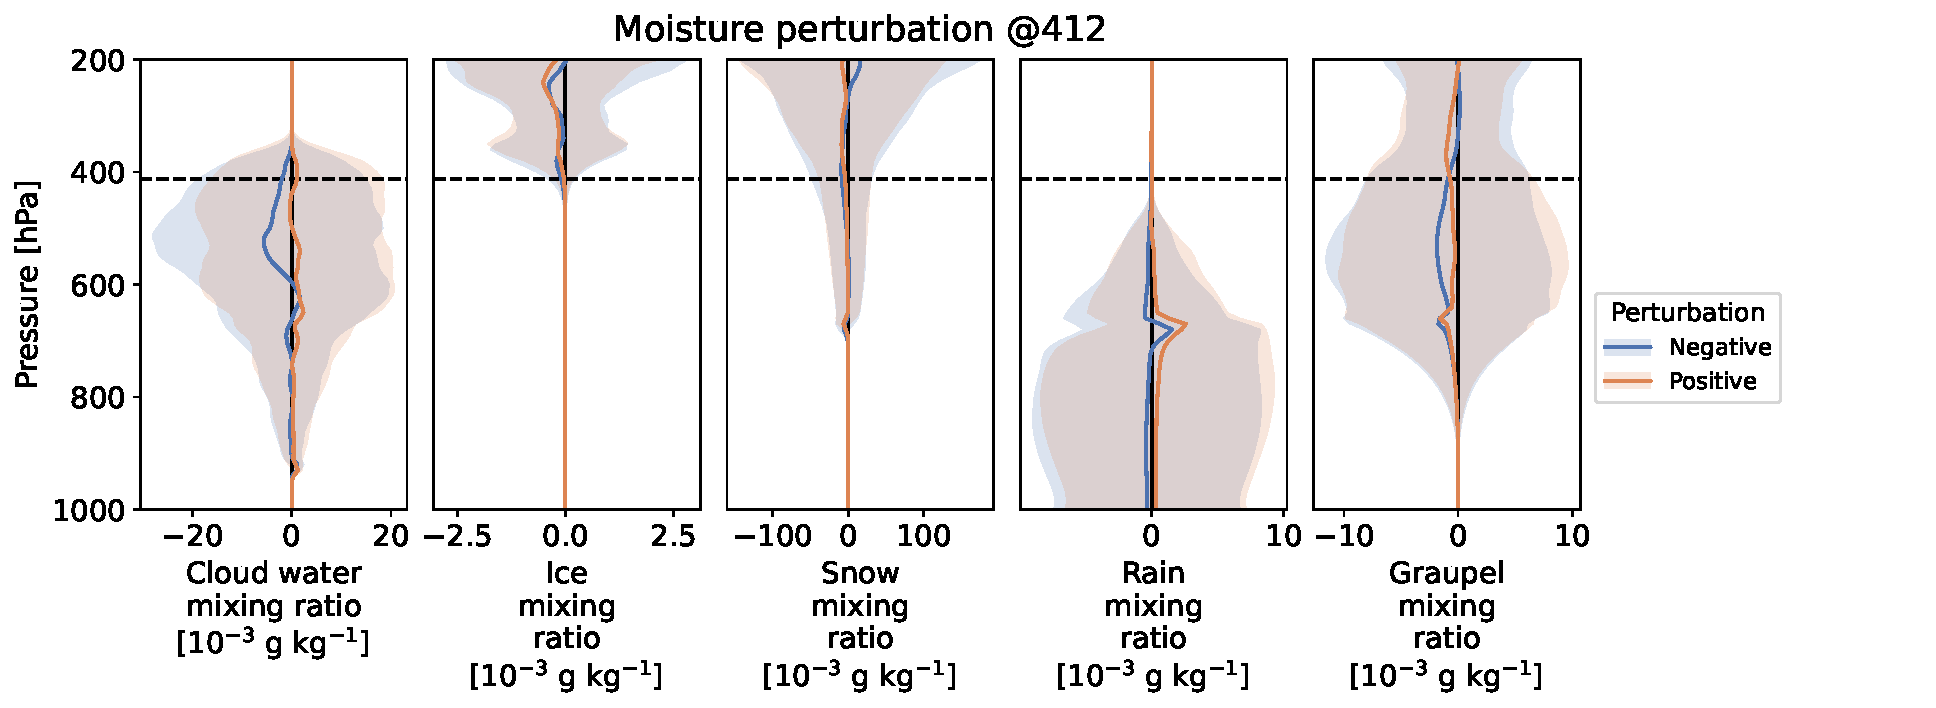
\includegraphics[width=\textwidth]{figures/pert_var_q_0.0002_@412}
    \caption{As in Figure \ref{fig:var_T_412} but for a water vapour mixing ratio perturbation of 0.2 g kg$^{-1}$ at 412 hPa.}
    \label{fig:var_q_412}
\end{figure}

\begin{figure}[pth]
    \noindent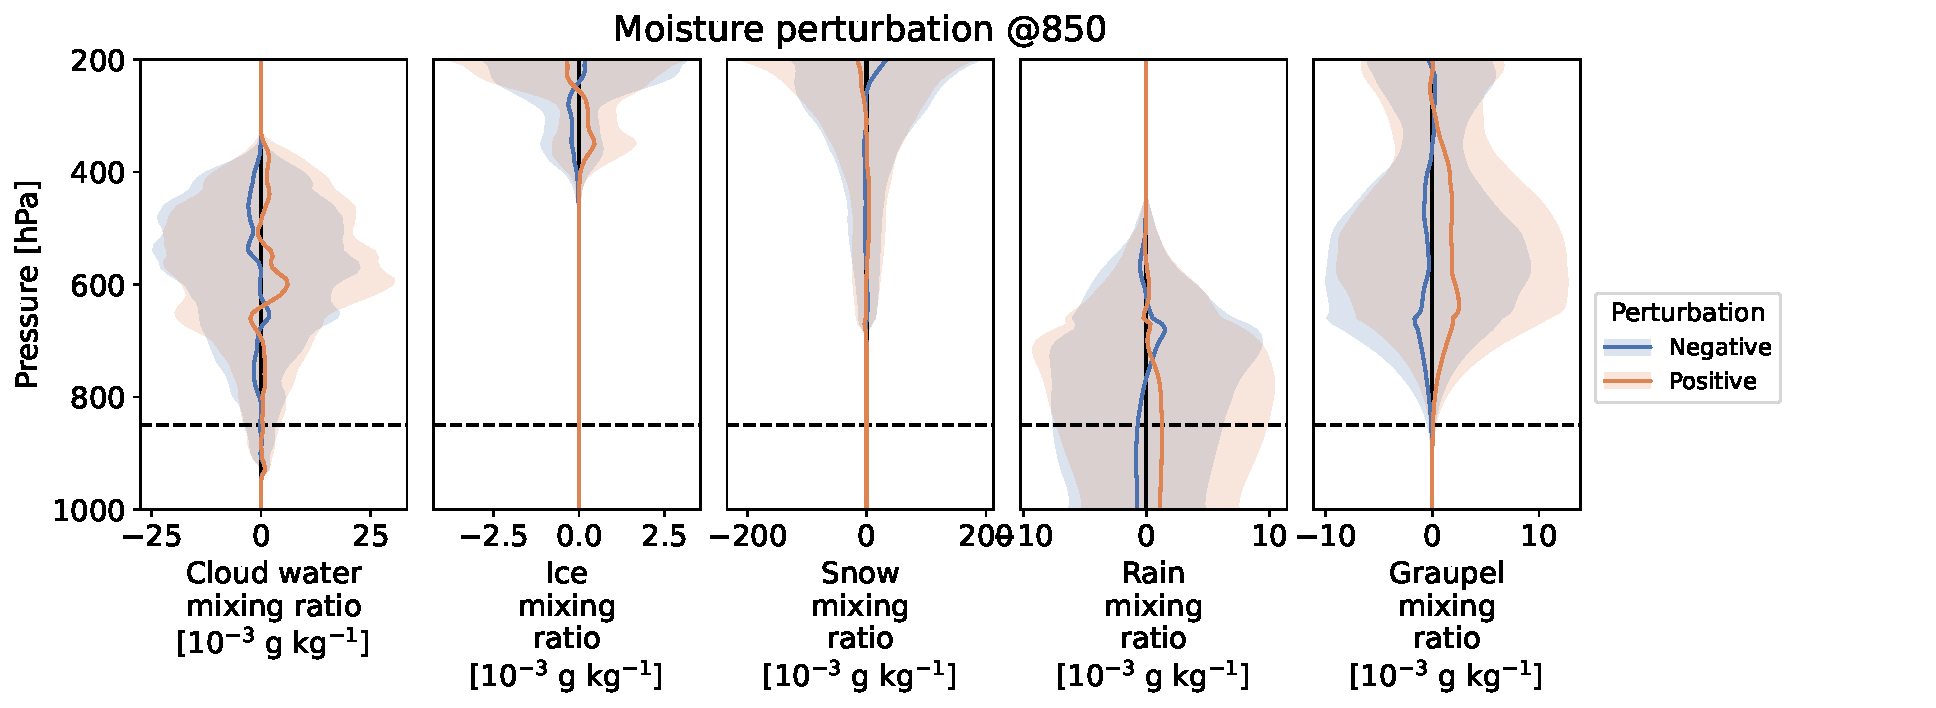
\includegraphics[width=\textwidth]{figures/pert_var_q_0.0002_@850}
    \caption{As in Figure \ref{fig:var_q_412} but for a water vapour mixing ratio perturbation of 0.2 g kg$^{-1}$ at 850 hPa.}
    \label{fig:var_q_850}
\end{figure}

\end{document}
